\documentclass[12pt]{article}

\usepackage[utf8]{inputenc}
\usepackage[T1]{fontenc}
\usepackage[spanish]{babel}
\usepackage{cmbright}
\usepackage{lmodern}
\usepackage{geometry}
\usepackage{tikz}
\usetikzlibrary{positioning,calc,math,arrows.meta,decorations.markings,intersections}
\usepackage{hyperref}
\usepackage[bf,sf,pagestyles]{titlesec}
\usepackage{titling}
\usepackage[runin]{abstract}
\usepackage[font={footnotesize, sf}, labelfont=bf]{caption} 
\usepackage{siunitx}
\usepackage{graphicx}
\usepackage{booktabs}
\usepackage{amsmath,amssymb}
\usepackage[spanish,sort]{cleveref}
\usepackage{enumitem}

\geometry{
	a4paper,
	right = 2.5cm,
	left = 2.5cm,
	bottom = 3cm,
	top = 3cm
}

\newcommand{\sfbright}{\fontfamily{cmbr}\selectfont}
\renewcommand{\familydefault}{\rmdefault}
\renewcommand{\sfdefault}{cmbr}
\renewcommand{\arraystretch}{1.4}

\hypersetup{
	colorlinks,
	linkcolor = {red!50!blue},
	citecolor = {red!50!blue},
	linktoc = page
}

\numberwithin{table}{section}
\numberwithin{figure}{section}
\numberwithin{equation}{section}

\graphicspath{{./figs/}}

% Unitats
\sisetup{
	inter-unit-product = \ensuremath{ \, },
	allow-number-unit-breaks = true,
	math-celsius = {}^{\circ}\kern-\scriptspace C,
	detect-family = true,
	mode = text,
	list-final-separator = { y },
	list-pair-separator = { y },
	list-units = single,
	separate-uncertainty = true
}

\DeclareUnicodeCharacter{2212}{-}

\newcommand{\Z}{\mathbb{Z}}
\newcommand{\N}{\mathbb{N}}
\newcommand{\R}{\mathbb{R}}
\newcommand{\Ry}{\mathit{Ry}}
\newcommand{\conv}[2]{\filldraw[fill = white!50!-red, fill opacity = 0.5, draw = -red!] (#1,0) ellipse [x radius = 0.1, y radius = #2];}
\newcommand{\data}[3]{\SI{#1 \pm #2}{#3}}
\newcommand{\unc}[2]{\ensuremath{{}\pm \SI{#1}{#2}}}
\DeclareMathOperator{\gr}{gr}
\newcommand{\abs}[1]{\left\lvert #1 \right\rvert}
\newcommand{\inn}[2]{\left\langle #1 , #2 \right\rangle}
\newcommand{\parbreak}{
	\begin{center}
		--- $\ast$ ---
	\end{center} 
}
\makeatletter
\newcommand*{\defeq}{\mathrel{\rlap{%
			\raisebox{0.3ex}{$\m@th\cdot$}}%
		\raisebox{-0.3ex}{$\m@th\cdot$}}%
	=
}
\makeatother

\newpagestyle{pagina}{
	\headrule
	\sethead*{\sffamily \bfseries Práctica 5}{}{\theauthor}
	\footrule
	\setfoot*{}{}{\sffamily \thepage}
}
\renewpagestyle{plain}{
	\footrule
	\setfoot*{}{}{\sffamily \thepage}
}
\pagestyle{pagina}

\title{\sffamily {\bfseries Práctica 5:} Polarización de la luz}
\author{\sffamily B2 2: Arnau Mas, Alejandro Plaza}
\date{\sffamily 28 de marzo de 2019}

\begin{document}
\maketitle
\renewcommand{\abstractname}{\sffamily \bfseries Resumen:}
\begin{abstract}
Abstract aquí
\end{abstract}
\hrule

\section{Objetivos}
En esta práctica se pretende estudiar el fenómeno de la polarización de la luz, ---que muestra que la luz es una onda transversal---, y diversos modos de causarlo.

Se estudiará la polarización por absorción selectiva de diversos materiales, por reflexión, por dispersión Rayleigh en la luz proveniente del cielo y por birrefringencia en láminas retardadoras.

Por último se comprobará la ley de Malus para la intensidad de luz que atraviesa dos polaroides.

\section{Polarización por dicroísmo}
La polarización por dicroísmo tiene lugar cuando la luz atraviesa una lámina de un material que absorbe una componente y transmite la perpendicular. Normalmente estas láminas consisten en cadenas rectilíneas de moléculas que permiten a los electrones moverse en una sola dirección. Si esta dirección es la vertical, los electrones interactuarán con la componente de la onda cuyo campo eléctrico oscile en el eje vertical, pues el que oscila en el eje horizontal no puede ejercer trabajo sobre los electrones, ya que estos no se desplazan en la dirección horizontal. Así pues los electrones de la lámina absorben la componente vertical del campo eléctrico y transmiten la componente horizontal.

Se apunta a una pantalla con una fuente de luz y se coloca un polarizador HN-22 entre ambas. El resultado es una leve disminución de la intensidad de la luz que llega a la pantalla. Al girar el polarizador no se observa ningún cambio, pues se está cambiando la dirección de polarización de la luz que llega a la pantalla pero no su intensidad.

La disminución de intensidad es un indicio de que la luz se ha polarizado, pero no es una prueba, pues podría por ejemplo absorberse una fracción de la luz igual para todas las direcciones. Para comprobar que efectivamente la luz sale polarizada se coloca entre el polaroide y la pantalla otro polaroide HN-38. al girar el segundo polaroide la intensidad va aumentando y disminuyendo. Cuando la pantalla está oscura es porque los ejes de transmisión de ambos polaroides son perpendiculares. El primer polaroide deja pasar luz únicamente en una dirección, que es justo la dirección que absorbe el segundo. Por lo tanto no llega luz a la pantalla y se ve oscura. Sin embargo, la oscuridad no es total, ya que los polarizadores no son ideales: tansmiten un poco de luz en la dirección de absorción y viceversa. Este fenómeno pone en evidencia que la luz que sale de los polaroides está efectivamente polarizada.

Ahora se cambia el polaroide HN-38 por uno HN-22, de manera que los dos polariodes tienen las mismas curvas de transmitancias. Estas curvas se encuentran en la figura \ref{P5transmitancias}. En este caso cuando los ejes de transmisión son perpendiculares se ve una oscuridad más intensa porque la transmitancia del polaroide HN-22 en el eje de absorción es mucho menor que la del HN-38. La intensidad cuando los ejes son paralelos es parecida con el polaroide HN-38 y el HN-22 porque tienen transmitancias similares en el eje de transmisión.

\begin{figure}[!ht]
\begin{center}
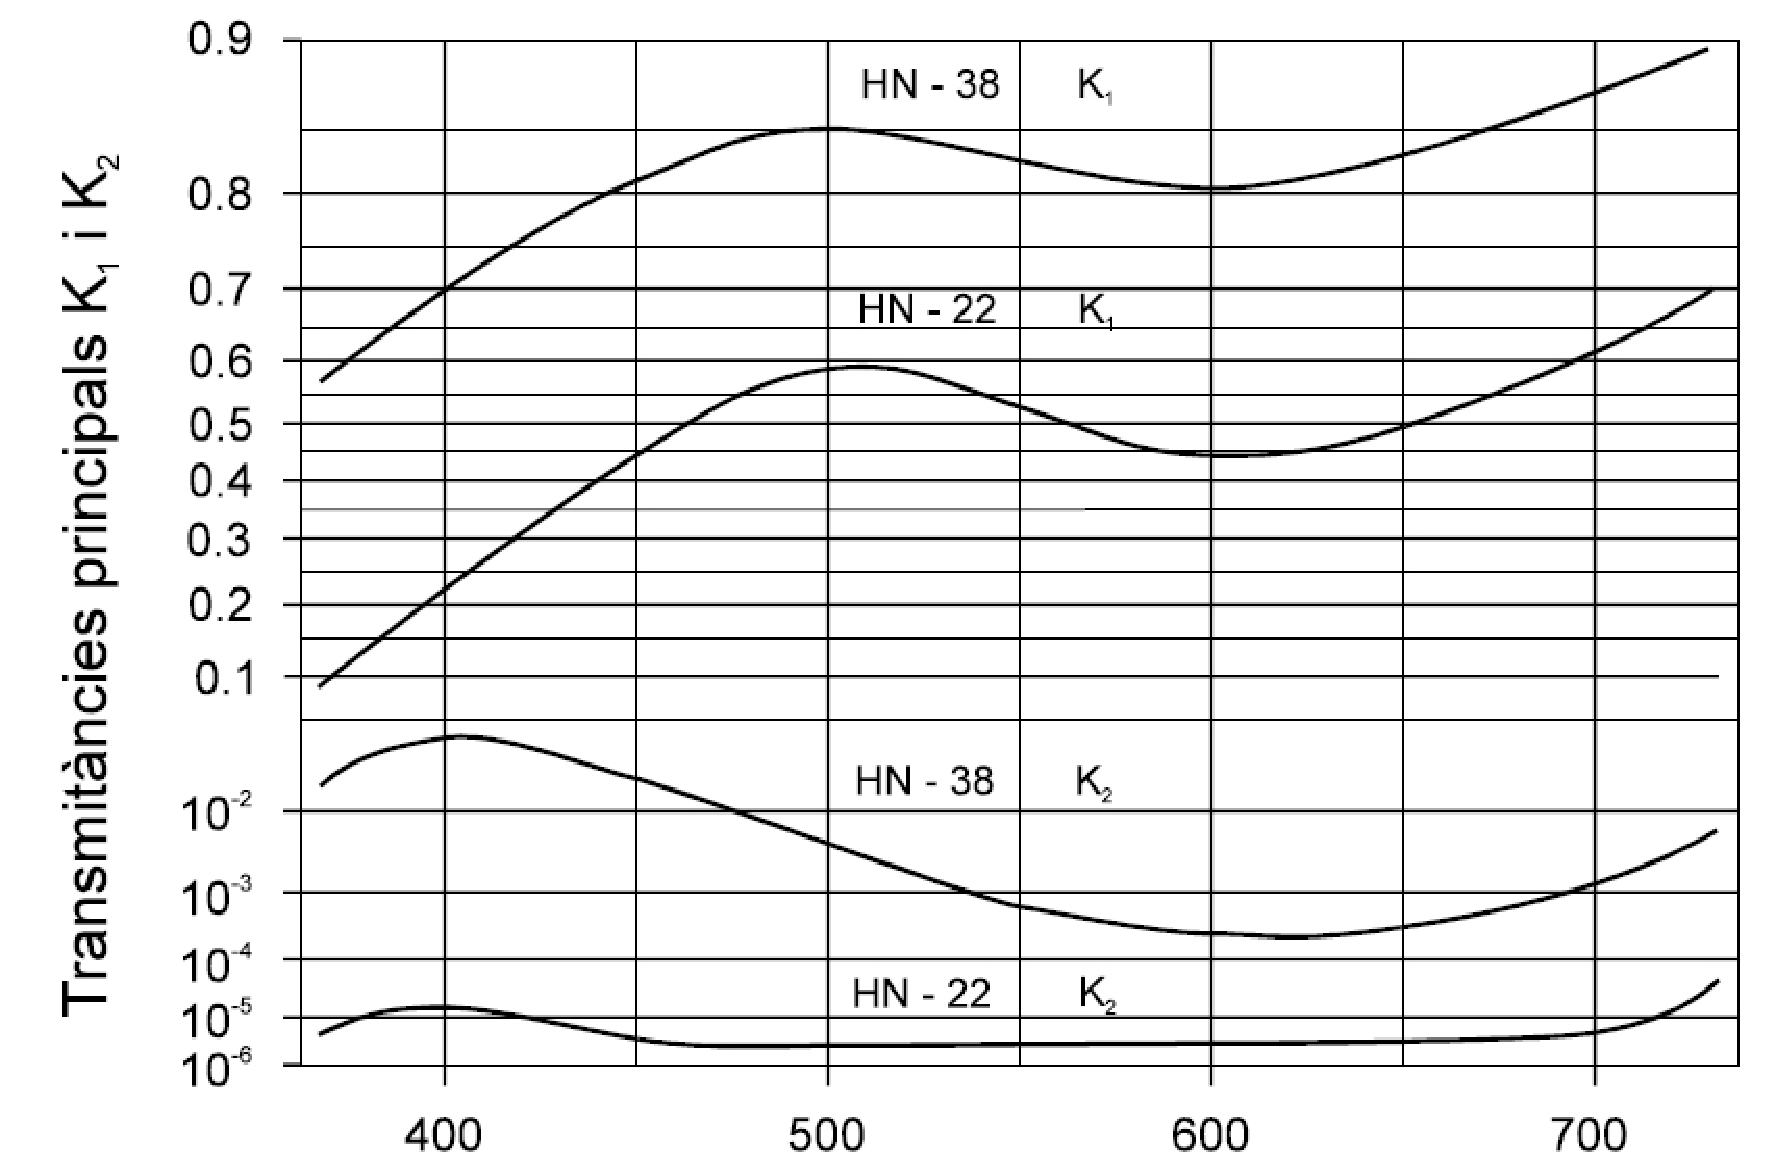
\includegraphics[width=10cm]{P5Transmitancias.pdf}
\caption{Gráficas de las transmitancias principales $K_1$ y $K_2$ en los ejes de transmisión y absorción respectivamente de los polarizadores HN-22 y HN-38 en función de la longitud de onda.}\label{P5transmitancias}
\end{center}
\end{figure}

Uno de los polarizadores tiene el eje de transmisión marcado. El eje de transmisión del otro se puede determinar girándolo hasta obtener la posición en la que la intensidad que llega a la pantalla es mínima. En este punto el eje de transmisión es el perpendicular al del otro polarizador ---cuyo eje de transmisión es conocido---. Este método es más preciso que girar el polarizador hasta obtener intensidad máxima ---siendo igual la dirección de transmisión de ambos polaroides--- porque se determina con mayor exactitud el ángulo de intensidad mínima que la máxima.

En la figura \ref{P5transmitancias} se ve que las transmitancias dependen de la longitud de onda. Para poner de manifiesto esta dependencia se colocan un filtro verde y otro rojo en la fuente de luz. Cuando los ejes son paralelos no se ve mucha diferencia, pero cuando son perpendiculares la luz que llega a la pantalla es menos intensa con el filtro verde que con el rojo. Si observamos la curva de $K_1$ del HN-22 la transmitancia es similar para longiudes de onda alrededor de los \SI{500}{nm} (verde) y de los \SI{700}{nm} (rojo). Sin embargo $K_2$ es bastante mayor para el rojo que el verde (obsérvese que del $10^{-1}$ hacia abajo la escala es logarítmica: pequeños cambios en el eje $y$ son grandes cambios de transmitancia).

Ahora se disponen los polarizadores con los ejes de transmisión cruzados y se colocan objetos entre ambos polarizadores. Se coloca asimismo una lente para proyectar los objetos sobre la pantalla. Este sistema se llama polariscopio.

Si se pone una lámina de vidrio no ocurre nada. La luz sale del vidrio tal cual ha entrado. No cambia su polarización. Por lo tanto se ve oscura la pantalla. Si se pone papel, sin embargo, sí que se ve algo de luz porque la luz polarizada que llega al papel se dispersa en él y sale despolarizada. Así la luz que llega al segundo polarizador tiene una componente no nula en el eje de transmisión. Independientemente de la orientación del papel o de los polarizadores se ve lpantalla iluminada.

Cuando se pone celofán se ilumina la pantalla según el ángulo de orientación. Cuando se gira se puede conseguir que se ilumine la pantalla. Si se orienta para ver el máximo de intensidad, para que vuelva a dejar de pasar la luz se ha de girar 90º. Esto se explica porque el celofán cambia la orientación de la polarización de la luz, de modo que si antes llegaba la luz oscilando perpendicular al eje de transmisión del segundo polarizador, con el celofán se puede cambiar la orientación de la polarización para que la luz llegue al segundo polarizador con el campo eléctrico oscilando en la dirección de transmisión.

También se puso una pequeña lámina de plástico con varios trozos de cinta adhesiva simple. Se observaron los distintos trozos de diferentes colores como muestra la figura \ref{P5colorines}. El celo modifica la orientación de la polarización de la luz, pero no afecta todas las longitudes de onda por igual: cada una gira su polarización por separado. Por eso algunas longitudes de onda llegan paralelas al eje de transmisión proyectándose sobre la pantalla y otras llegan perpendiculares siendo absorbidas. Además cada capa modifica la polarización y por lo tanto según la cantidad de capas de cinta que haya se ve de un color u otro. Al girar el plástico se ve cómo cambian los colores.

\begin{figure}[!ht]
	\centering
	\begin{minipage}{0.45\textwidth}
		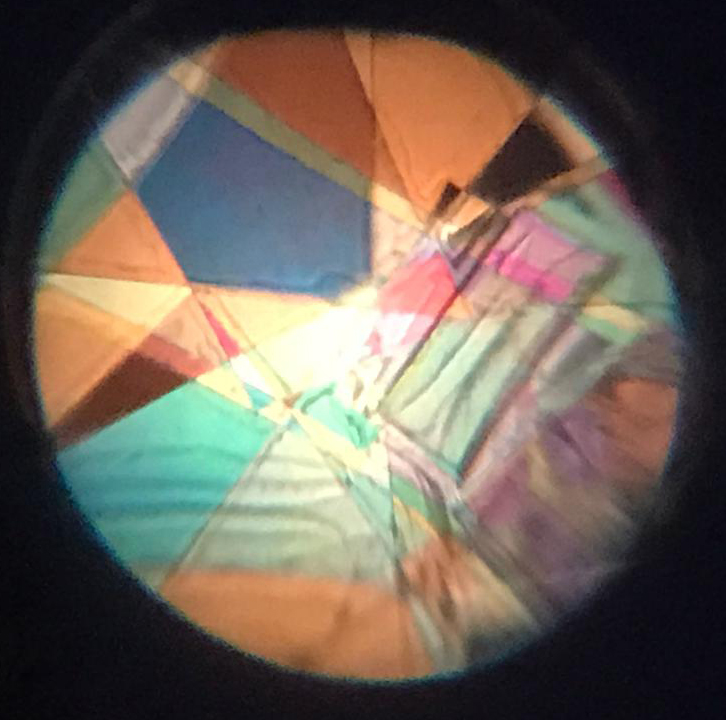
\includegraphics[scale = 0.25]{P5Celo1.jpg}
	\end{minipage}
	\begin{minipage}{0.45\textwidth}
		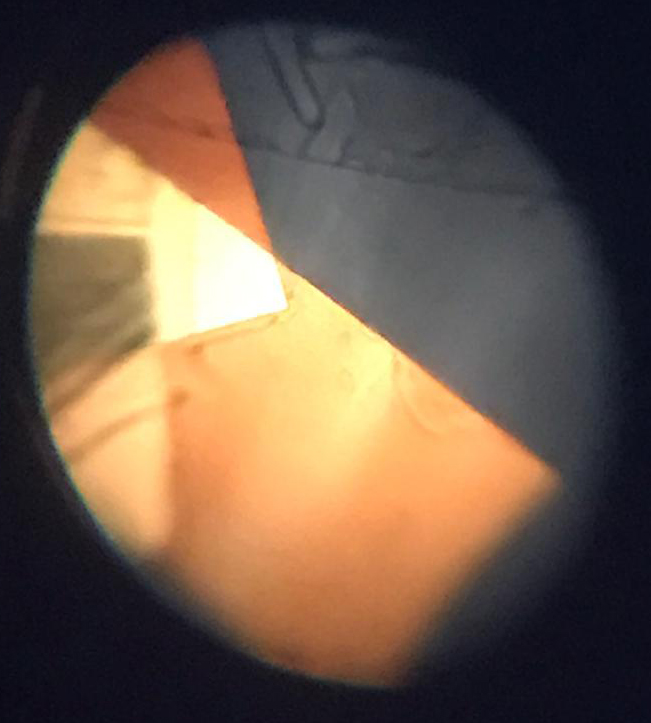
\includegraphics[scale = 0.25]{P5Celo2.jpg}
	\end{minipage}
\caption{Fotografías de la la pantalla con cinta adhesiva en el polariscopio.}\label{P5colorines}
\end{figure}

Por último se coloca una caja de un CD, que es un plástico rígido, en el polariscopio. Se observan diversos colores en la pantalla como con la cinta adhesiva. Al presionar el plástico, los colores cambian, lo cual se puede explicar porque al sufrir esfuerzos el plástico cambia la orientación de las diversas longitudes de onda de la luz polarizada.

\section{Polarización por reflexión}


\section{Verificación de la ley de Malus}
A continuación verificaremos experimentalmente la ley de Malus. Esta ley da la intensidad transmitida a través de dos polarizadoes en términos de su orientación relativa. Si los dos polarizadores son iguales entonces se puede demostrar que la intensidad transmitida de un haz monocromático que los atraviesa es
\begin{equation*}
	I(\theta) = K_1K_2I_0 + \tfrac{1}{2}K_1(K_1 - 2K_2)I_0 (\cos{\theta})^2 
\end{equation*}
donde \( K_1 \) y \( K_2 \) son las transmitancias principales de los polarizadores. Ahora bien, si la luz incidente no es monocromática y las transmitancias del polarizador dependen de la longitud de onda entonces debemos integrar sobre la distribución espectral de la luz incidente. Supondremos, pues, que estamos tratando con un polarizador ideal, por lo que la ley de Malus se reduce a la forma más conocida:
\begin{equation} \label{eqn:malus}
	I(\theta) = \tfrac{1}{2} (\cos{\theta})^2.
\end{equation}

\begin{figure}[htb]
	\centering \small \sffamily
	%% Creator: Matplotlib, PGF backend
%%
%% To include the figure in your LaTeX document, write
%%   \input{<filename>.pgf}
%%
%% Make sure the required packages are loaded in your preamble
%%   \usepackage{pgf}
%%
%% Figures using additional raster images can only be included by \input if
%% they are in the same directory as the main LaTeX file. For loading figures
%% from other directories you can use the `import` package
%%   \usepackage{import}
%% and then include the figures with
%%   \import{<path to file>}{<filename>.pgf}
%%
%% Matplotlib used the following preamble
%%   \usepackage{siunitx}
%%   \usepackage[utf8]{inputenc}
%%   \usepackage{fontspec}
%%
\begingroup%
\makeatletter%
\begin{pgfpicture}%
\pgfpathrectangle{\pgfpointorigin}{\pgfqpoint{5.000000in}{3.500000in}}%
\pgfusepath{use as bounding box, clip}%
\begin{pgfscope}%
\pgfsetbuttcap%
\pgfsetmiterjoin%
\definecolor{currentfill}{rgb}{1.000000,1.000000,1.000000}%
\pgfsetfillcolor{currentfill}%
\pgfsetlinewidth{0.000000pt}%
\definecolor{currentstroke}{rgb}{1.000000,1.000000,1.000000}%
\pgfsetstrokecolor{currentstroke}%
\pgfsetdash{}{0pt}%
\pgfpathmoveto{\pgfqpoint{0.000000in}{0.000000in}}%
\pgfpathlineto{\pgfqpoint{5.000000in}{0.000000in}}%
\pgfpathlineto{\pgfqpoint{5.000000in}{3.500000in}}%
\pgfpathlineto{\pgfqpoint{0.000000in}{3.500000in}}%
\pgfpathclose%
\pgfusepath{fill}%
\end{pgfscope}%
\begin{pgfscope}%
\pgfsetbuttcap%
\pgfsetmiterjoin%
\definecolor{currentfill}{rgb}{1.000000,1.000000,1.000000}%
\pgfsetfillcolor{currentfill}%
\pgfsetlinewidth{0.000000pt}%
\definecolor{currentstroke}{rgb}{0.000000,0.000000,0.000000}%
\pgfsetstrokecolor{currentstroke}%
\pgfsetstrokeopacity{0.000000}%
\pgfsetdash{}{0pt}%
\pgfpathmoveto{\pgfqpoint{0.625000in}{0.437500in}}%
\pgfpathlineto{\pgfqpoint{4.500000in}{0.437500in}}%
\pgfpathlineto{\pgfqpoint{4.500000in}{3.080000in}}%
\pgfpathlineto{\pgfqpoint{0.625000in}{3.080000in}}%
\pgfpathclose%
\pgfusepath{fill}%
\end{pgfscope}%
\begin{pgfscope}%
\pgfpathrectangle{\pgfqpoint{0.625000in}{0.437500in}}{\pgfqpoint{3.875000in}{2.642500in}}%
\pgfusepath{clip}%
\pgfsetrectcap%
\pgfsetroundjoin%
\pgfsetlinewidth{0.803000pt}%
\definecolor{currentstroke}{rgb}{0.690196,0.690196,0.690196}%
\pgfsetstrokecolor{currentstroke}%
\pgfsetdash{}{0pt}%
\pgfpathmoveto{\pgfqpoint{1.035985in}{0.437500in}}%
\pgfpathlineto{\pgfqpoint{1.035985in}{3.080000in}}%
\pgfusepath{stroke}%
\end{pgfscope}%
\begin{pgfscope}%
\pgfsetbuttcap%
\pgfsetroundjoin%
\definecolor{currentfill}{rgb}{0.000000,0.000000,0.000000}%
\pgfsetfillcolor{currentfill}%
\pgfsetlinewidth{0.803000pt}%
\definecolor{currentstroke}{rgb}{0.000000,0.000000,0.000000}%
\pgfsetstrokecolor{currentstroke}%
\pgfsetdash{}{0pt}%
\pgfsys@defobject{currentmarker}{\pgfqpoint{0.000000in}{-0.048611in}}{\pgfqpoint{0.000000in}{0.000000in}}{%
\pgfpathmoveto{\pgfqpoint{0.000000in}{0.000000in}}%
\pgfpathlineto{\pgfqpoint{0.000000in}{-0.048611in}}%
\pgfusepath{stroke,fill}%
}%
\begin{pgfscope}%
\pgfsys@transformshift{1.035985in}{0.437500in}%
\pgfsys@useobject{currentmarker}{}%
\end{pgfscope}%
\end{pgfscope}%
\begin{pgfscope}%
\pgftext[x=1.035985in,y=0.340278in,,top]{\sffamily\fontsize{10.000000}{12.000000}\selectfont −75}%
\end{pgfscope}%
\begin{pgfscope}%
\pgfpathrectangle{\pgfqpoint{0.625000in}{0.437500in}}{\pgfqpoint{3.875000in}{2.642500in}}%
\pgfusepath{clip}%
\pgfsetrectcap%
\pgfsetroundjoin%
\pgfsetlinewidth{0.803000pt}%
\definecolor{currentstroke}{rgb}{0.690196,0.690196,0.690196}%
\pgfsetstrokecolor{currentstroke}%
\pgfsetdash{}{0pt}%
\pgfpathmoveto{\pgfqpoint{1.525253in}{0.437500in}}%
\pgfpathlineto{\pgfqpoint{1.525253in}{3.080000in}}%
\pgfusepath{stroke}%
\end{pgfscope}%
\begin{pgfscope}%
\pgfsetbuttcap%
\pgfsetroundjoin%
\definecolor{currentfill}{rgb}{0.000000,0.000000,0.000000}%
\pgfsetfillcolor{currentfill}%
\pgfsetlinewidth{0.803000pt}%
\definecolor{currentstroke}{rgb}{0.000000,0.000000,0.000000}%
\pgfsetstrokecolor{currentstroke}%
\pgfsetdash{}{0pt}%
\pgfsys@defobject{currentmarker}{\pgfqpoint{0.000000in}{-0.048611in}}{\pgfqpoint{0.000000in}{0.000000in}}{%
\pgfpathmoveto{\pgfqpoint{0.000000in}{0.000000in}}%
\pgfpathlineto{\pgfqpoint{0.000000in}{-0.048611in}}%
\pgfusepath{stroke,fill}%
}%
\begin{pgfscope}%
\pgfsys@transformshift{1.525253in}{0.437500in}%
\pgfsys@useobject{currentmarker}{}%
\end{pgfscope}%
\end{pgfscope}%
\begin{pgfscope}%
\pgftext[x=1.525253in,y=0.340278in,,top]{\sffamily\fontsize{10.000000}{12.000000}\selectfont −50}%
\end{pgfscope}%
\begin{pgfscope}%
\pgfpathrectangle{\pgfqpoint{0.625000in}{0.437500in}}{\pgfqpoint{3.875000in}{2.642500in}}%
\pgfusepath{clip}%
\pgfsetrectcap%
\pgfsetroundjoin%
\pgfsetlinewidth{0.803000pt}%
\definecolor{currentstroke}{rgb}{0.690196,0.690196,0.690196}%
\pgfsetstrokecolor{currentstroke}%
\pgfsetdash{}{0pt}%
\pgfpathmoveto{\pgfqpoint{2.014520in}{0.437500in}}%
\pgfpathlineto{\pgfqpoint{2.014520in}{3.080000in}}%
\pgfusepath{stroke}%
\end{pgfscope}%
\begin{pgfscope}%
\pgfsetbuttcap%
\pgfsetroundjoin%
\definecolor{currentfill}{rgb}{0.000000,0.000000,0.000000}%
\pgfsetfillcolor{currentfill}%
\pgfsetlinewidth{0.803000pt}%
\definecolor{currentstroke}{rgb}{0.000000,0.000000,0.000000}%
\pgfsetstrokecolor{currentstroke}%
\pgfsetdash{}{0pt}%
\pgfsys@defobject{currentmarker}{\pgfqpoint{0.000000in}{-0.048611in}}{\pgfqpoint{0.000000in}{0.000000in}}{%
\pgfpathmoveto{\pgfqpoint{0.000000in}{0.000000in}}%
\pgfpathlineto{\pgfqpoint{0.000000in}{-0.048611in}}%
\pgfusepath{stroke,fill}%
}%
\begin{pgfscope}%
\pgfsys@transformshift{2.014520in}{0.437500in}%
\pgfsys@useobject{currentmarker}{}%
\end{pgfscope}%
\end{pgfscope}%
\begin{pgfscope}%
\pgftext[x=2.014520in,y=0.340278in,,top]{\sffamily\fontsize{10.000000}{12.000000}\selectfont −25}%
\end{pgfscope}%
\begin{pgfscope}%
\pgfpathrectangle{\pgfqpoint{0.625000in}{0.437500in}}{\pgfqpoint{3.875000in}{2.642500in}}%
\pgfusepath{clip}%
\pgfsetrectcap%
\pgfsetroundjoin%
\pgfsetlinewidth{0.803000pt}%
\definecolor{currentstroke}{rgb}{0.690196,0.690196,0.690196}%
\pgfsetstrokecolor{currentstroke}%
\pgfsetdash{}{0pt}%
\pgfpathmoveto{\pgfqpoint{2.503788in}{0.437500in}}%
\pgfpathlineto{\pgfqpoint{2.503788in}{3.080000in}}%
\pgfusepath{stroke}%
\end{pgfscope}%
\begin{pgfscope}%
\pgfsetbuttcap%
\pgfsetroundjoin%
\definecolor{currentfill}{rgb}{0.000000,0.000000,0.000000}%
\pgfsetfillcolor{currentfill}%
\pgfsetlinewidth{0.803000pt}%
\definecolor{currentstroke}{rgb}{0.000000,0.000000,0.000000}%
\pgfsetstrokecolor{currentstroke}%
\pgfsetdash{}{0pt}%
\pgfsys@defobject{currentmarker}{\pgfqpoint{0.000000in}{-0.048611in}}{\pgfqpoint{0.000000in}{0.000000in}}{%
\pgfpathmoveto{\pgfqpoint{0.000000in}{0.000000in}}%
\pgfpathlineto{\pgfqpoint{0.000000in}{-0.048611in}}%
\pgfusepath{stroke,fill}%
}%
\begin{pgfscope}%
\pgfsys@transformshift{2.503788in}{0.437500in}%
\pgfsys@useobject{currentmarker}{}%
\end{pgfscope}%
\end{pgfscope}%
\begin{pgfscope}%
\pgftext[x=2.503788in,y=0.340278in,,top]{\sffamily\fontsize{10.000000}{12.000000}\selectfont 0}%
\end{pgfscope}%
\begin{pgfscope}%
\pgfpathrectangle{\pgfqpoint{0.625000in}{0.437500in}}{\pgfqpoint{3.875000in}{2.642500in}}%
\pgfusepath{clip}%
\pgfsetrectcap%
\pgfsetroundjoin%
\pgfsetlinewidth{0.803000pt}%
\definecolor{currentstroke}{rgb}{0.690196,0.690196,0.690196}%
\pgfsetstrokecolor{currentstroke}%
\pgfsetdash{}{0pt}%
\pgfpathmoveto{\pgfqpoint{2.993056in}{0.437500in}}%
\pgfpathlineto{\pgfqpoint{2.993056in}{3.080000in}}%
\pgfusepath{stroke}%
\end{pgfscope}%
\begin{pgfscope}%
\pgfsetbuttcap%
\pgfsetroundjoin%
\definecolor{currentfill}{rgb}{0.000000,0.000000,0.000000}%
\pgfsetfillcolor{currentfill}%
\pgfsetlinewidth{0.803000pt}%
\definecolor{currentstroke}{rgb}{0.000000,0.000000,0.000000}%
\pgfsetstrokecolor{currentstroke}%
\pgfsetdash{}{0pt}%
\pgfsys@defobject{currentmarker}{\pgfqpoint{0.000000in}{-0.048611in}}{\pgfqpoint{0.000000in}{0.000000in}}{%
\pgfpathmoveto{\pgfqpoint{0.000000in}{0.000000in}}%
\pgfpathlineto{\pgfqpoint{0.000000in}{-0.048611in}}%
\pgfusepath{stroke,fill}%
}%
\begin{pgfscope}%
\pgfsys@transformshift{2.993056in}{0.437500in}%
\pgfsys@useobject{currentmarker}{}%
\end{pgfscope}%
\end{pgfscope}%
\begin{pgfscope}%
\pgftext[x=2.993056in,y=0.340278in,,top]{\sffamily\fontsize{10.000000}{12.000000}\selectfont 25}%
\end{pgfscope}%
\begin{pgfscope}%
\pgfpathrectangle{\pgfqpoint{0.625000in}{0.437500in}}{\pgfqpoint{3.875000in}{2.642500in}}%
\pgfusepath{clip}%
\pgfsetrectcap%
\pgfsetroundjoin%
\pgfsetlinewidth{0.803000pt}%
\definecolor{currentstroke}{rgb}{0.690196,0.690196,0.690196}%
\pgfsetstrokecolor{currentstroke}%
\pgfsetdash{}{0pt}%
\pgfpathmoveto{\pgfqpoint{3.482323in}{0.437500in}}%
\pgfpathlineto{\pgfqpoint{3.482323in}{3.080000in}}%
\pgfusepath{stroke}%
\end{pgfscope}%
\begin{pgfscope}%
\pgfsetbuttcap%
\pgfsetroundjoin%
\definecolor{currentfill}{rgb}{0.000000,0.000000,0.000000}%
\pgfsetfillcolor{currentfill}%
\pgfsetlinewidth{0.803000pt}%
\definecolor{currentstroke}{rgb}{0.000000,0.000000,0.000000}%
\pgfsetstrokecolor{currentstroke}%
\pgfsetdash{}{0pt}%
\pgfsys@defobject{currentmarker}{\pgfqpoint{0.000000in}{-0.048611in}}{\pgfqpoint{0.000000in}{0.000000in}}{%
\pgfpathmoveto{\pgfqpoint{0.000000in}{0.000000in}}%
\pgfpathlineto{\pgfqpoint{0.000000in}{-0.048611in}}%
\pgfusepath{stroke,fill}%
}%
\begin{pgfscope}%
\pgfsys@transformshift{3.482323in}{0.437500in}%
\pgfsys@useobject{currentmarker}{}%
\end{pgfscope}%
\end{pgfscope}%
\begin{pgfscope}%
\pgftext[x=3.482323in,y=0.340278in,,top]{\sffamily\fontsize{10.000000}{12.000000}\selectfont 50}%
\end{pgfscope}%
\begin{pgfscope}%
\pgfpathrectangle{\pgfqpoint{0.625000in}{0.437500in}}{\pgfqpoint{3.875000in}{2.642500in}}%
\pgfusepath{clip}%
\pgfsetrectcap%
\pgfsetroundjoin%
\pgfsetlinewidth{0.803000pt}%
\definecolor{currentstroke}{rgb}{0.690196,0.690196,0.690196}%
\pgfsetstrokecolor{currentstroke}%
\pgfsetdash{}{0pt}%
\pgfpathmoveto{\pgfqpoint{3.971591in}{0.437500in}}%
\pgfpathlineto{\pgfqpoint{3.971591in}{3.080000in}}%
\pgfusepath{stroke}%
\end{pgfscope}%
\begin{pgfscope}%
\pgfsetbuttcap%
\pgfsetroundjoin%
\definecolor{currentfill}{rgb}{0.000000,0.000000,0.000000}%
\pgfsetfillcolor{currentfill}%
\pgfsetlinewidth{0.803000pt}%
\definecolor{currentstroke}{rgb}{0.000000,0.000000,0.000000}%
\pgfsetstrokecolor{currentstroke}%
\pgfsetdash{}{0pt}%
\pgfsys@defobject{currentmarker}{\pgfqpoint{0.000000in}{-0.048611in}}{\pgfqpoint{0.000000in}{0.000000in}}{%
\pgfpathmoveto{\pgfqpoint{0.000000in}{0.000000in}}%
\pgfpathlineto{\pgfqpoint{0.000000in}{-0.048611in}}%
\pgfusepath{stroke,fill}%
}%
\begin{pgfscope}%
\pgfsys@transformshift{3.971591in}{0.437500in}%
\pgfsys@useobject{currentmarker}{}%
\end{pgfscope}%
\end{pgfscope}%
\begin{pgfscope}%
\pgftext[x=3.971591in,y=0.340278in,,top]{\sffamily\fontsize{10.000000}{12.000000}\selectfont 75}%
\end{pgfscope}%
\begin{pgfscope}%
\pgfpathrectangle{\pgfqpoint{0.625000in}{0.437500in}}{\pgfqpoint{3.875000in}{2.642500in}}%
\pgfusepath{clip}%
\pgfsetrectcap%
\pgfsetroundjoin%
\pgfsetlinewidth{0.803000pt}%
\definecolor{currentstroke}{rgb}{0.690196,0.690196,0.690196}%
\pgfsetstrokecolor{currentstroke}%
\pgfsetdash{}{0pt}%
\pgfpathmoveto{\pgfqpoint{4.460859in}{0.437500in}}%
\pgfpathlineto{\pgfqpoint{4.460859in}{3.080000in}}%
\pgfusepath{stroke}%
\end{pgfscope}%
\begin{pgfscope}%
\pgfsetbuttcap%
\pgfsetroundjoin%
\definecolor{currentfill}{rgb}{0.000000,0.000000,0.000000}%
\pgfsetfillcolor{currentfill}%
\pgfsetlinewidth{0.803000pt}%
\definecolor{currentstroke}{rgb}{0.000000,0.000000,0.000000}%
\pgfsetstrokecolor{currentstroke}%
\pgfsetdash{}{0pt}%
\pgfsys@defobject{currentmarker}{\pgfqpoint{0.000000in}{-0.048611in}}{\pgfqpoint{0.000000in}{0.000000in}}{%
\pgfpathmoveto{\pgfqpoint{0.000000in}{0.000000in}}%
\pgfpathlineto{\pgfqpoint{0.000000in}{-0.048611in}}%
\pgfusepath{stroke,fill}%
}%
\begin{pgfscope}%
\pgfsys@transformshift{4.460859in}{0.437500in}%
\pgfsys@useobject{currentmarker}{}%
\end{pgfscope}%
\end{pgfscope}%
\begin{pgfscope}%
\pgftext[x=4.460859in,y=0.340278in,,top]{\sffamily\fontsize{10.000000}{12.000000}\selectfont 100}%
\end{pgfscope}%
\begin{pgfscope}%
\pgftext[x=2.562500in,y=0.161389in,,top]{\sffamily\fontsize{10.000000}{12.000000}\selectfont \( \theta \, (\si{\degree}) \)}%
\end{pgfscope}%
\begin{pgfscope}%
\pgfpathrectangle{\pgfqpoint{0.625000in}{0.437500in}}{\pgfqpoint{3.875000in}{2.642500in}}%
\pgfusepath{clip}%
\pgfsetrectcap%
\pgfsetroundjoin%
\pgfsetlinewidth{0.803000pt}%
\definecolor{currentstroke}{rgb}{0.690196,0.690196,0.690196}%
\pgfsetstrokecolor{currentstroke}%
\pgfsetdash{}{0pt}%
\pgfpathmoveto{\pgfqpoint{0.625000in}{0.557614in}}%
\pgfpathlineto{\pgfqpoint{4.500000in}{0.557614in}}%
\pgfusepath{stroke}%
\end{pgfscope}%
\begin{pgfscope}%
\pgfsetbuttcap%
\pgfsetroundjoin%
\definecolor{currentfill}{rgb}{0.000000,0.000000,0.000000}%
\pgfsetfillcolor{currentfill}%
\pgfsetlinewidth{0.803000pt}%
\definecolor{currentstroke}{rgb}{0.000000,0.000000,0.000000}%
\pgfsetstrokecolor{currentstroke}%
\pgfsetdash{}{0pt}%
\pgfsys@defobject{currentmarker}{\pgfqpoint{-0.048611in}{0.000000in}}{\pgfqpoint{0.000000in}{0.000000in}}{%
\pgfpathmoveto{\pgfqpoint{0.000000in}{0.000000in}}%
\pgfpathlineto{\pgfqpoint{-0.048611in}{0.000000in}}%
\pgfusepath{stroke,fill}%
}%
\begin{pgfscope}%
\pgfsys@transformshift{0.625000in}{0.557614in}%
\pgfsys@useobject{currentmarker}{}%
\end{pgfscope}%
\end{pgfscope}%
\begin{pgfscope}%
\pgftext[x=0.350278in,y=0.509419in,left,base]{\sffamily\fontsize{10.000000}{12.000000}\selectfont 0.0}%
\end{pgfscope}%
\begin{pgfscope}%
\pgfpathrectangle{\pgfqpoint{0.625000in}{0.437500in}}{\pgfqpoint{3.875000in}{2.642500in}}%
\pgfusepath{clip}%
\pgfsetrectcap%
\pgfsetroundjoin%
\pgfsetlinewidth{0.803000pt}%
\definecolor{currentstroke}{rgb}{0.690196,0.690196,0.690196}%
\pgfsetstrokecolor{currentstroke}%
\pgfsetdash{}{0pt}%
\pgfpathmoveto{\pgfqpoint{0.625000in}{1.033311in}}%
\pgfpathlineto{\pgfqpoint{4.500000in}{1.033311in}}%
\pgfusepath{stroke}%
\end{pgfscope}%
\begin{pgfscope}%
\pgfsetbuttcap%
\pgfsetroundjoin%
\definecolor{currentfill}{rgb}{0.000000,0.000000,0.000000}%
\pgfsetfillcolor{currentfill}%
\pgfsetlinewidth{0.803000pt}%
\definecolor{currentstroke}{rgb}{0.000000,0.000000,0.000000}%
\pgfsetstrokecolor{currentstroke}%
\pgfsetdash{}{0pt}%
\pgfsys@defobject{currentmarker}{\pgfqpoint{-0.048611in}{0.000000in}}{\pgfqpoint{0.000000in}{0.000000in}}{%
\pgfpathmoveto{\pgfqpoint{0.000000in}{0.000000in}}%
\pgfpathlineto{\pgfqpoint{-0.048611in}{0.000000in}}%
\pgfusepath{stroke,fill}%
}%
\begin{pgfscope}%
\pgfsys@transformshift{0.625000in}{1.033311in}%
\pgfsys@useobject{currentmarker}{}%
\end{pgfscope}%
\end{pgfscope}%
\begin{pgfscope}%
\pgftext[x=0.350278in,y=0.985117in,left,base]{\sffamily\fontsize{10.000000}{12.000000}\selectfont 0.2}%
\end{pgfscope}%
\begin{pgfscope}%
\pgfpathrectangle{\pgfqpoint{0.625000in}{0.437500in}}{\pgfqpoint{3.875000in}{2.642500in}}%
\pgfusepath{clip}%
\pgfsetrectcap%
\pgfsetroundjoin%
\pgfsetlinewidth{0.803000pt}%
\definecolor{currentstroke}{rgb}{0.690196,0.690196,0.690196}%
\pgfsetstrokecolor{currentstroke}%
\pgfsetdash{}{0pt}%
\pgfpathmoveto{\pgfqpoint{0.625000in}{1.509009in}}%
\pgfpathlineto{\pgfqpoint{4.500000in}{1.509009in}}%
\pgfusepath{stroke}%
\end{pgfscope}%
\begin{pgfscope}%
\pgfsetbuttcap%
\pgfsetroundjoin%
\definecolor{currentfill}{rgb}{0.000000,0.000000,0.000000}%
\pgfsetfillcolor{currentfill}%
\pgfsetlinewidth{0.803000pt}%
\definecolor{currentstroke}{rgb}{0.000000,0.000000,0.000000}%
\pgfsetstrokecolor{currentstroke}%
\pgfsetdash{}{0pt}%
\pgfsys@defobject{currentmarker}{\pgfqpoint{-0.048611in}{0.000000in}}{\pgfqpoint{0.000000in}{0.000000in}}{%
\pgfpathmoveto{\pgfqpoint{0.000000in}{0.000000in}}%
\pgfpathlineto{\pgfqpoint{-0.048611in}{0.000000in}}%
\pgfusepath{stroke,fill}%
}%
\begin{pgfscope}%
\pgfsys@transformshift{0.625000in}{1.509009in}%
\pgfsys@useobject{currentmarker}{}%
\end{pgfscope}%
\end{pgfscope}%
\begin{pgfscope}%
\pgftext[x=0.350278in,y=1.460814in,left,base]{\sffamily\fontsize{10.000000}{12.000000}\selectfont 0.4}%
\end{pgfscope}%
\begin{pgfscope}%
\pgfpathrectangle{\pgfqpoint{0.625000in}{0.437500in}}{\pgfqpoint{3.875000in}{2.642500in}}%
\pgfusepath{clip}%
\pgfsetrectcap%
\pgfsetroundjoin%
\pgfsetlinewidth{0.803000pt}%
\definecolor{currentstroke}{rgb}{0.690196,0.690196,0.690196}%
\pgfsetstrokecolor{currentstroke}%
\pgfsetdash{}{0pt}%
\pgfpathmoveto{\pgfqpoint{0.625000in}{1.984706in}}%
\pgfpathlineto{\pgfqpoint{4.500000in}{1.984706in}}%
\pgfusepath{stroke}%
\end{pgfscope}%
\begin{pgfscope}%
\pgfsetbuttcap%
\pgfsetroundjoin%
\definecolor{currentfill}{rgb}{0.000000,0.000000,0.000000}%
\pgfsetfillcolor{currentfill}%
\pgfsetlinewidth{0.803000pt}%
\definecolor{currentstroke}{rgb}{0.000000,0.000000,0.000000}%
\pgfsetstrokecolor{currentstroke}%
\pgfsetdash{}{0pt}%
\pgfsys@defobject{currentmarker}{\pgfqpoint{-0.048611in}{0.000000in}}{\pgfqpoint{0.000000in}{0.000000in}}{%
\pgfpathmoveto{\pgfqpoint{0.000000in}{0.000000in}}%
\pgfpathlineto{\pgfqpoint{-0.048611in}{0.000000in}}%
\pgfusepath{stroke,fill}%
}%
\begin{pgfscope}%
\pgfsys@transformshift{0.625000in}{1.984706in}%
\pgfsys@useobject{currentmarker}{}%
\end{pgfscope}%
\end{pgfscope}%
\begin{pgfscope}%
\pgftext[x=0.350278in,y=1.936512in,left,base]{\sffamily\fontsize{10.000000}{12.000000}\selectfont 0.6}%
\end{pgfscope}%
\begin{pgfscope}%
\pgfpathrectangle{\pgfqpoint{0.625000in}{0.437500in}}{\pgfqpoint{3.875000in}{2.642500in}}%
\pgfusepath{clip}%
\pgfsetrectcap%
\pgfsetroundjoin%
\pgfsetlinewidth{0.803000pt}%
\definecolor{currentstroke}{rgb}{0.690196,0.690196,0.690196}%
\pgfsetstrokecolor{currentstroke}%
\pgfsetdash{}{0pt}%
\pgfpathmoveto{\pgfqpoint{0.625000in}{2.460404in}}%
\pgfpathlineto{\pgfqpoint{4.500000in}{2.460404in}}%
\pgfusepath{stroke}%
\end{pgfscope}%
\begin{pgfscope}%
\pgfsetbuttcap%
\pgfsetroundjoin%
\definecolor{currentfill}{rgb}{0.000000,0.000000,0.000000}%
\pgfsetfillcolor{currentfill}%
\pgfsetlinewidth{0.803000pt}%
\definecolor{currentstroke}{rgb}{0.000000,0.000000,0.000000}%
\pgfsetstrokecolor{currentstroke}%
\pgfsetdash{}{0pt}%
\pgfsys@defobject{currentmarker}{\pgfqpoint{-0.048611in}{0.000000in}}{\pgfqpoint{0.000000in}{0.000000in}}{%
\pgfpathmoveto{\pgfqpoint{0.000000in}{0.000000in}}%
\pgfpathlineto{\pgfqpoint{-0.048611in}{0.000000in}}%
\pgfusepath{stroke,fill}%
}%
\begin{pgfscope}%
\pgfsys@transformshift{0.625000in}{2.460404in}%
\pgfsys@useobject{currentmarker}{}%
\end{pgfscope}%
\end{pgfscope}%
\begin{pgfscope}%
\pgftext[x=0.350278in,y=2.412209in,left,base]{\sffamily\fontsize{10.000000}{12.000000}\selectfont 0.8}%
\end{pgfscope}%
\begin{pgfscope}%
\pgfpathrectangle{\pgfqpoint{0.625000in}{0.437500in}}{\pgfqpoint{3.875000in}{2.642500in}}%
\pgfusepath{clip}%
\pgfsetrectcap%
\pgfsetroundjoin%
\pgfsetlinewidth{0.803000pt}%
\definecolor{currentstroke}{rgb}{0.690196,0.690196,0.690196}%
\pgfsetstrokecolor{currentstroke}%
\pgfsetdash{}{0pt}%
\pgfpathmoveto{\pgfqpoint{0.625000in}{2.936101in}}%
\pgfpathlineto{\pgfqpoint{4.500000in}{2.936101in}}%
\pgfusepath{stroke}%
\end{pgfscope}%
\begin{pgfscope}%
\pgfsetbuttcap%
\pgfsetroundjoin%
\definecolor{currentfill}{rgb}{0.000000,0.000000,0.000000}%
\pgfsetfillcolor{currentfill}%
\pgfsetlinewidth{0.803000pt}%
\definecolor{currentstroke}{rgb}{0.000000,0.000000,0.000000}%
\pgfsetstrokecolor{currentstroke}%
\pgfsetdash{}{0pt}%
\pgfsys@defobject{currentmarker}{\pgfqpoint{-0.048611in}{0.000000in}}{\pgfqpoint{0.000000in}{0.000000in}}{%
\pgfpathmoveto{\pgfqpoint{0.000000in}{0.000000in}}%
\pgfpathlineto{\pgfqpoint{-0.048611in}{0.000000in}}%
\pgfusepath{stroke,fill}%
}%
\begin{pgfscope}%
\pgfsys@transformshift{0.625000in}{2.936101in}%
\pgfsys@useobject{currentmarker}{}%
\end{pgfscope}%
\end{pgfscope}%
\begin{pgfscope}%
\pgftext[x=0.350278in,y=2.887907in,left,base]{\sffamily\fontsize{10.000000}{12.000000}\selectfont 1.0}%
\end{pgfscope}%
\begin{pgfscope}%
\pgftext[x=0.294722in,y=1.758750in,,bottom,rotate=90.000000]{\sffamily\fontsize{10.000000}{12.000000}\selectfont \( I \, (\si{\mW}) \)}%
\end{pgfscope}%
\begin{pgfscope}%
\pgfpathrectangle{\pgfqpoint{0.625000in}{0.437500in}}{\pgfqpoint{3.875000in}{2.642500in}}%
\pgfusepath{clip}%
\pgfsetbuttcap%
\pgfsetroundjoin%
\definecolor{currentfill}{rgb}{0.678431,0.847059,0.901961}%
\pgfsetfillcolor{currentfill}%
\pgfsetlinewidth{1.003750pt}%
\definecolor{currentstroke}{rgb}{0.121569,0.466667,0.705882}%
\pgfsetstrokecolor{currentstroke}%
\pgfsetdash{}{0pt}%
\pgfsys@defobject{currentmarker}{\pgfqpoint{-0.048611in}{-0.048611in}}{\pgfqpoint{0.048611in}{0.048611in}}{%
\pgfpathmoveto{\pgfqpoint{-0.048611in}{0.000000in}}%
\pgfpathlineto{\pgfqpoint{0.048611in}{0.000000in}}%
\pgfpathmoveto{\pgfqpoint{0.000000in}{-0.048611in}}%
\pgfpathlineto{\pgfqpoint{0.000000in}{0.048611in}}%
\pgfusepath{stroke,fill}%
}%
\begin{pgfscope}%
\pgfsys@transformshift{0.801136in}{0.557614in}%
\pgfsys@useobject{currentmarker}{}%
\end{pgfscope}%
\begin{pgfscope}%
\pgfsys@transformshift{0.996843in}{0.700323in}%
\pgfsys@useobject{currentmarker}{}%
\end{pgfscope}%
\begin{pgfscope}%
\pgfsys@transformshift{1.192551in}{0.914387in}%
\pgfsys@useobject{currentmarker}{}%
\end{pgfscope}%
\begin{pgfscope}%
\pgfsys@transformshift{1.388258in}{1.271160in}%
\pgfsys@useobject{currentmarker}{}%
\end{pgfscope}%
\begin{pgfscope}%
\pgfsys@transformshift{1.583965in}{1.651718in}%
\pgfsys@useobject{currentmarker}{}%
\end{pgfscope}%
\begin{pgfscope}%
\pgfsys@transformshift{1.779672in}{2.103631in}%
\pgfsys@useobject{currentmarker}{}%
\end{pgfscope}%
\begin{pgfscope}%
\pgfsys@transformshift{1.975379in}{2.436619in}%
\pgfsys@useobject{currentmarker}{}%
\end{pgfscope}%
\begin{pgfscope}%
\pgfsys@transformshift{2.171086in}{2.722038in}%
\pgfsys@useobject{currentmarker}{}%
\end{pgfscope}%
\begin{pgfscope}%
\pgfsys@transformshift{2.366793in}{2.912317in}%
\pgfsys@useobject{currentmarker}{}%
\end{pgfscope}%
\begin{pgfscope}%
\pgfsys@transformshift{2.249369in}{2.817177in}%
\pgfsys@useobject{currentmarker}{}%
\end{pgfscope}%
\begin{pgfscope}%
\pgfsys@transformshift{2.210227in}{2.769607in}%
\pgfsys@useobject{currentmarker}{}%
\end{pgfscope}%
\begin{pgfscope}%
\pgfsys@transformshift{2.288510in}{2.864747in}%
\pgfsys@useobject{currentmarker}{}%
\end{pgfscope}%
\begin{pgfscope}%
\pgfsys@transformshift{2.327652in}{2.888532in}%
\pgfsys@useobject{currentmarker}{}%
\end{pgfscope}%
\begin{pgfscope}%
\pgfsys@transformshift{2.405934in}{2.936101in}%
\pgfsys@useobject{currentmarker}{}%
\end{pgfscope}%
\begin{pgfscope}%
\pgfsys@transformshift{2.445076in}{2.936101in}%
\pgfsys@useobject{currentmarker}{}%
\end{pgfscope}%
\begin{pgfscope}%
\pgfsys@transformshift{2.484217in}{2.959886in}%
\pgfsys@useobject{currentmarker}{}%
\end{pgfscope}%
\begin{pgfscope}%
\pgfsys@transformshift{2.523359in}{2.959886in}%
\pgfsys@useobject{currentmarker}{}%
\end{pgfscope}%
\begin{pgfscope}%
\pgfsys@transformshift{2.562500in}{2.936101in}%
\pgfsys@useobject{currentmarker}{}%
\end{pgfscope}%
\begin{pgfscope}%
\pgfsys@transformshift{2.601641in}{2.936101in}%
\pgfsys@useobject{currentmarker}{}%
\end{pgfscope}%
\begin{pgfscope}%
\pgfsys@transformshift{2.640783in}{2.912317in}%
\pgfsys@useobject{currentmarker}{}%
\end{pgfscope}%
\begin{pgfscope}%
\pgfsys@transformshift{2.679924in}{2.888532in}%
\pgfsys@useobject{currentmarker}{}%
\end{pgfscope}%
\begin{pgfscope}%
\pgfsys@transformshift{2.719066in}{2.864747in}%
\pgfsys@useobject{currentmarker}{}%
\end{pgfscope}%
\begin{pgfscope}%
\pgfsys@transformshift{2.758207in}{2.840962in}%
\pgfsys@useobject{currentmarker}{}%
\end{pgfscope}%
\begin{pgfscope}%
\pgfsys@transformshift{2.797348in}{2.793392in}%
\pgfsys@useobject{currentmarker}{}%
\end{pgfscope}%
\begin{pgfscope}%
\pgfsys@transformshift{2.836490in}{2.745822in}%
\pgfsys@useobject{currentmarker}{}%
\end{pgfscope}%
\begin{pgfscope}%
\pgfsys@transformshift{2.875631in}{2.698253in}%
\pgfsys@useobject{currentmarker}{}%
\end{pgfscope}%
\begin{pgfscope}%
\pgfsys@transformshift{2.914773in}{2.650683in}%
\pgfsys@useobject{currentmarker}{}%
\end{pgfscope}%
\begin{pgfscope}%
\pgfsys@transformshift{2.953914in}{2.603113in}%
\pgfsys@useobject{currentmarker}{}%
\end{pgfscope}%
\begin{pgfscope}%
\pgfsys@transformshift{3.149621in}{2.270125in}%
\pgfsys@useobject{currentmarker}{}%
\end{pgfscope}%
\begin{pgfscope}%
\pgfsys@transformshift{3.345328in}{1.889567in}%
\pgfsys@useobject{currentmarker}{}%
\end{pgfscope}%
\begin{pgfscope}%
\pgfsys@transformshift{3.541035in}{1.461439in}%
\pgfsys@useobject{currentmarker}{}%
\end{pgfscope}%
\begin{pgfscope}%
\pgfsys@transformshift{3.736742in}{1.057096in}%
\pgfsys@useobject{currentmarker}{}%
\end{pgfscope}%
\begin{pgfscope}%
\pgfsys@transformshift{3.932449in}{0.771678in}%
\pgfsys@useobject{currentmarker}{}%
\end{pgfscope}%
\begin{pgfscope}%
\pgfsys@transformshift{4.128157in}{0.605183in}%
\pgfsys@useobject{currentmarker}{}%
\end{pgfscope}%
\begin{pgfscope}%
\pgfsys@transformshift{4.323864in}{0.557614in}%
\pgfsys@useobject{currentmarker}{}%
\end{pgfscope}%
\end{pgfscope}%
\begin{pgfscope}%
\pgfsetrectcap%
\pgfsetmiterjoin%
\pgfsetlinewidth{0.803000pt}%
\definecolor{currentstroke}{rgb}{0.000000,0.000000,0.000000}%
\pgfsetstrokecolor{currentstroke}%
\pgfsetdash{}{0pt}%
\pgfpathmoveto{\pgfqpoint{0.625000in}{0.437500in}}%
\pgfpathlineto{\pgfqpoint{0.625000in}{3.080000in}}%
\pgfusepath{stroke}%
\end{pgfscope}%
\begin{pgfscope}%
\pgfsetrectcap%
\pgfsetmiterjoin%
\pgfsetlinewidth{0.803000pt}%
\definecolor{currentstroke}{rgb}{0.000000,0.000000,0.000000}%
\pgfsetstrokecolor{currentstroke}%
\pgfsetdash{}{0pt}%
\pgfpathmoveto{\pgfqpoint{4.500000in}{0.437500in}}%
\pgfpathlineto{\pgfqpoint{4.500000in}{3.080000in}}%
\pgfusepath{stroke}%
\end{pgfscope}%
\begin{pgfscope}%
\pgfsetrectcap%
\pgfsetmiterjoin%
\pgfsetlinewidth{0.803000pt}%
\definecolor{currentstroke}{rgb}{0.000000,0.000000,0.000000}%
\pgfsetstrokecolor{currentstroke}%
\pgfsetdash{}{0pt}%
\pgfpathmoveto{\pgfqpoint{0.625000in}{0.437500in}}%
\pgfpathlineto{\pgfqpoint{4.500000in}{0.437500in}}%
\pgfusepath{stroke}%
\end{pgfscope}%
\begin{pgfscope}%
\pgfsetrectcap%
\pgfsetmiterjoin%
\pgfsetlinewidth{0.803000pt}%
\definecolor{currentstroke}{rgb}{0.000000,0.000000,0.000000}%
\pgfsetstrokecolor{currentstroke}%
\pgfsetdash{}{0pt}%
\pgfpathmoveto{\pgfqpoint{0.625000in}{3.080000in}}%
\pgfpathlineto{\pgfqpoint{4.500000in}{3.080000in}}%
\pgfusepath{stroke}%
\end{pgfscope}%
\end{pgfpicture}%
\makeatother%
\endgroup%

	\caption{Representación de las medidas de la intensidad transmitida en función del ángulo entre los polarizadores. La incertidumbre en \( \theta \) es de \unc{2}{\degree}, y la de \( I \) es de \unc{0.01}{mW} por lo que no se pueden apreciar en el gráfico.}
	\label{fig:malus-1}
\end{figure}

Para tomar las medidas disponemos de dos polarizadores iguales y dos lentes para colimar el haz antes y después de atravesar los polarizadores. Finalmetne disponemos de un fotómetro para medir la intensidad transmitida. Para empezar a tomar medidas colocamos los polarizadores con los ejes perpendiculares de manera que la intensidad transmitida sea lo más cercana a 0 posible y fijamos el 0 del fotómetro. Aún así, el rango de ángulos en el que la lectura era inferior al umbral de tolerancia del fotómetro es considerablemente grande, por lo que es preciso corregir las medidas del ángulo a posteriori. Tomamos medidas cada \SI{10}{\degree} y cada \SI{2}{\degree} alrededor del máximo de intensidad. 

En la \cref{fig:malus-1} se muestran las medidas. Para determinar el ángulo relativo se tomó como origen el pico de intensidad. Las lecturas de intensidad máxima, de \SI{1.01}{mW}, se dieron en \SI{166}{\degree} y \SI{168}{\degree} donde este ángulo corresponde a la lectura en el goniómetro del segundo polarizador. Así pues se tomó el origen en la media de estos valores. 

Podemos ver como los datos se ajustan bien a la forma de un coseno cuadrado. Para determinar exactamente las constantes de proporcionalidad hacemos una regresión lineal de la forma
\begin{equation} \label{eqn:regresión}
	I(\theta) = A + B(\cos{\theta})^2.
\end{equation}
Con la función \texttt{linregress} del módulo \textsf{SciPy} obtenemos unos valores para los parámetros de
\begin{equation} \label{eqn:parametros}
	\begin{gathered}
		A = \data{0.004}{0.002}{mW} \\
		B = \data{1.002}{0.003}{mW}
	\end{gathered}
\end{equation}
y un coeficiente de correlación \( r^2 = \num{0.9997} \). El ajuste está representado en la \cref{fig:regr}.

\begin{figure}[htb]
	\centering \small \sffamily
	%% Creator: Matplotlib, PGF backend
%%
%% To include the figure in your LaTeX document, write
%%   \input{<filename>.pgf}
%%
%% Make sure the required packages are loaded in your preamble
%%   \usepackage{pgf}
%%
%% Figures using additional raster images can only be included by \input if
%% they are in the same directory as the main LaTeX file. For loading figures
%% from other directories you can use the `import` package
%%   \usepackage{import}
%% and then include the figures with
%%   \import{<path to file>}{<filename>.pgf}
%%
%% Matplotlib used the following preamble
%%   \usepackage{siunitx}
%%   \usepackage[utf8]{inputenc}
%%   \usepackage{fontspec}
%%
\begingroup%
\makeatletter%
\begin{pgfpicture}%
\pgfpathrectangle{\pgfpointorigin}{\pgfqpoint{5.000000in}{3.500000in}}%
\pgfusepath{use as bounding box, clip}%
\begin{pgfscope}%
\pgfsetbuttcap%
\pgfsetmiterjoin%
\definecolor{currentfill}{rgb}{1.000000,1.000000,1.000000}%
\pgfsetfillcolor{currentfill}%
\pgfsetlinewidth{0.000000pt}%
\definecolor{currentstroke}{rgb}{1.000000,1.000000,1.000000}%
\pgfsetstrokecolor{currentstroke}%
\pgfsetdash{}{0pt}%
\pgfpathmoveto{\pgfqpoint{0.000000in}{0.000000in}}%
\pgfpathlineto{\pgfqpoint{5.000000in}{0.000000in}}%
\pgfpathlineto{\pgfqpoint{5.000000in}{3.500000in}}%
\pgfpathlineto{\pgfqpoint{0.000000in}{3.500000in}}%
\pgfpathclose%
\pgfusepath{fill}%
\end{pgfscope}%
\begin{pgfscope}%
\pgfsetbuttcap%
\pgfsetmiterjoin%
\definecolor{currentfill}{rgb}{1.000000,1.000000,1.000000}%
\pgfsetfillcolor{currentfill}%
\pgfsetlinewidth{0.000000pt}%
\definecolor{currentstroke}{rgb}{0.000000,0.000000,0.000000}%
\pgfsetstrokecolor{currentstroke}%
\pgfsetstrokeopacity{0.000000}%
\pgfsetdash{}{0pt}%
\pgfpathmoveto{\pgfqpoint{0.625000in}{0.437500in}}%
\pgfpathlineto{\pgfqpoint{4.500000in}{0.437500in}}%
\pgfpathlineto{\pgfqpoint{4.500000in}{3.080000in}}%
\pgfpathlineto{\pgfqpoint{0.625000in}{3.080000in}}%
\pgfpathclose%
\pgfusepath{fill}%
\end{pgfscope}%
\begin{pgfscope}%
\pgfpathrectangle{\pgfqpoint{0.625000in}{0.437500in}}{\pgfqpoint{3.875000in}{2.642500in}}%
\pgfusepath{clip}%
\pgfsetrectcap%
\pgfsetroundjoin%
\pgfsetlinewidth{0.803000pt}%
\definecolor{currentstroke}{rgb}{0.690196,0.690196,0.690196}%
\pgfsetstrokecolor{currentstroke}%
\pgfsetdash{}{0pt}%
\pgfpathmoveto{\pgfqpoint{0.801136in}{0.437500in}}%
\pgfpathlineto{\pgfqpoint{0.801136in}{3.080000in}}%
\pgfusepath{stroke}%
\end{pgfscope}%
\begin{pgfscope}%
\pgfsetbuttcap%
\pgfsetroundjoin%
\definecolor{currentfill}{rgb}{0.000000,0.000000,0.000000}%
\pgfsetfillcolor{currentfill}%
\pgfsetlinewidth{0.803000pt}%
\definecolor{currentstroke}{rgb}{0.000000,0.000000,0.000000}%
\pgfsetstrokecolor{currentstroke}%
\pgfsetdash{}{0pt}%
\pgfsys@defobject{currentmarker}{\pgfqpoint{0.000000in}{-0.048611in}}{\pgfqpoint{0.000000in}{0.000000in}}{%
\pgfpathmoveto{\pgfqpoint{0.000000in}{0.000000in}}%
\pgfpathlineto{\pgfqpoint{0.000000in}{-0.048611in}}%
\pgfusepath{stroke,fill}%
}%
\begin{pgfscope}%
\pgfsys@transformshift{0.801136in}{0.437500in}%
\pgfsys@useobject{currentmarker}{}%
\end{pgfscope}%
\end{pgfscope}%
\begin{pgfscope}%
\pgftext[x=0.801136in,y=0.340278in,,top]{\sffamily\fontsize{10.000000}{12.000000}\selectfont 0.0}%
\end{pgfscope}%
\begin{pgfscope}%
\pgfpathrectangle{\pgfqpoint{0.625000in}{0.437500in}}{\pgfqpoint{3.875000in}{2.642500in}}%
\pgfusepath{clip}%
\pgfsetrectcap%
\pgfsetroundjoin%
\pgfsetlinewidth{0.803000pt}%
\definecolor{currentstroke}{rgb}{0.690196,0.690196,0.690196}%
\pgfsetstrokecolor{currentstroke}%
\pgfsetdash{}{0pt}%
\pgfpathmoveto{\pgfqpoint{1.505896in}{0.437500in}}%
\pgfpathlineto{\pgfqpoint{1.505896in}{3.080000in}}%
\pgfusepath{stroke}%
\end{pgfscope}%
\begin{pgfscope}%
\pgfsetbuttcap%
\pgfsetroundjoin%
\definecolor{currentfill}{rgb}{0.000000,0.000000,0.000000}%
\pgfsetfillcolor{currentfill}%
\pgfsetlinewidth{0.803000pt}%
\definecolor{currentstroke}{rgb}{0.000000,0.000000,0.000000}%
\pgfsetstrokecolor{currentstroke}%
\pgfsetdash{}{0pt}%
\pgfsys@defobject{currentmarker}{\pgfqpoint{0.000000in}{-0.048611in}}{\pgfqpoint{0.000000in}{0.000000in}}{%
\pgfpathmoveto{\pgfqpoint{0.000000in}{0.000000in}}%
\pgfpathlineto{\pgfqpoint{0.000000in}{-0.048611in}}%
\pgfusepath{stroke,fill}%
}%
\begin{pgfscope}%
\pgfsys@transformshift{1.505896in}{0.437500in}%
\pgfsys@useobject{currentmarker}{}%
\end{pgfscope}%
\end{pgfscope}%
\begin{pgfscope}%
\pgftext[x=1.505896in,y=0.340278in,,top]{\sffamily\fontsize{10.000000}{12.000000}\selectfont 0.2}%
\end{pgfscope}%
\begin{pgfscope}%
\pgfpathrectangle{\pgfqpoint{0.625000in}{0.437500in}}{\pgfqpoint{3.875000in}{2.642500in}}%
\pgfusepath{clip}%
\pgfsetrectcap%
\pgfsetroundjoin%
\pgfsetlinewidth{0.803000pt}%
\definecolor{currentstroke}{rgb}{0.690196,0.690196,0.690196}%
\pgfsetstrokecolor{currentstroke}%
\pgfsetdash{}{0pt}%
\pgfpathmoveto{\pgfqpoint{2.210657in}{0.437500in}}%
\pgfpathlineto{\pgfqpoint{2.210657in}{3.080000in}}%
\pgfusepath{stroke}%
\end{pgfscope}%
\begin{pgfscope}%
\pgfsetbuttcap%
\pgfsetroundjoin%
\definecolor{currentfill}{rgb}{0.000000,0.000000,0.000000}%
\pgfsetfillcolor{currentfill}%
\pgfsetlinewidth{0.803000pt}%
\definecolor{currentstroke}{rgb}{0.000000,0.000000,0.000000}%
\pgfsetstrokecolor{currentstroke}%
\pgfsetdash{}{0pt}%
\pgfsys@defobject{currentmarker}{\pgfqpoint{0.000000in}{-0.048611in}}{\pgfqpoint{0.000000in}{0.000000in}}{%
\pgfpathmoveto{\pgfqpoint{0.000000in}{0.000000in}}%
\pgfpathlineto{\pgfqpoint{0.000000in}{-0.048611in}}%
\pgfusepath{stroke,fill}%
}%
\begin{pgfscope}%
\pgfsys@transformshift{2.210657in}{0.437500in}%
\pgfsys@useobject{currentmarker}{}%
\end{pgfscope}%
\end{pgfscope}%
\begin{pgfscope}%
\pgftext[x=2.210657in,y=0.340278in,,top]{\sffamily\fontsize{10.000000}{12.000000}\selectfont 0.4}%
\end{pgfscope}%
\begin{pgfscope}%
\pgfpathrectangle{\pgfqpoint{0.625000in}{0.437500in}}{\pgfqpoint{3.875000in}{2.642500in}}%
\pgfusepath{clip}%
\pgfsetrectcap%
\pgfsetroundjoin%
\pgfsetlinewidth{0.803000pt}%
\definecolor{currentstroke}{rgb}{0.690196,0.690196,0.690196}%
\pgfsetstrokecolor{currentstroke}%
\pgfsetdash{}{0pt}%
\pgfpathmoveto{\pgfqpoint{2.915417in}{0.437500in}}%
\pgfpathlineto{\pgfqpoint{2.915417in}{3.080000in}}%
\pgfusepath{stroke}%
\end{pgfscope}%
\begin{pgfscope}%
\pgfsetbuttcap%
\pgfsetroundjoin%
\definecolor{currentfill}{rgb}{0.000000,0.000000,0.000000}%
\pgfsetfillcolor{currentfill}%
\pgfsetlinewidth{0.803000pt}%
\definecolor{currentstroke}{rgb}{0.000000,0.000000,0.000000}%
\pgfsetstrokecolor{currentstroke}%
\pgfsetdash{}{0pt}%
\pgfsys@defobject{currentmarker}{\pgfqpoint{0.000000in}{-0.048611in}}{\pgfqpoint{0.000000in}{0.000000in}}{%
\pgfpathmoveto{\pgfqpoint{0.000000in}{0.000000in}}%
\pgfpathlineto{\pgfqpoint{0.000000in}{-0.048611in}}%
\pgfusepath{stroke,fill}%
}%
\begin{pgfscope}%
\pgfsys@transformshift{2.915417in}{0.437500in}%
\pgfsys@useobject{currentmarker}{}%
\end{pgfscope}%
\end{pgfscope}%
\begin{pgfscope}%
\pgftext[x=2.915417in,y=0.340278in,,top]{\sffamily\fontsize{10.000000}{12.000000}\selectfont 0.6}%
\end{pgfscope}%
\begin{pgfscope}%
\pgfpathrectangle{\pgfqpoint{0.625000in}{0.437500in}}{\pgfqpoint{3.875000in}{2.642500in}}%
\pgfusepath{clip}%
\pgfsetrectcap%
\pgfsetroundjoin%
\pgfsetlinewidth{0.803000pt}%
\definecolor{currentstroke}{rgb}{0.690196,0.690196,0.690196}%
\pgfsetstrokecolor{currentstroke}%
\pgfsetdash{}{0pt}%
\pgfpathmoveto{\pgfqpoint{3.620177in}{0.437500in}}%
\pgfpathlineto{\pgfqpoint{3.620177in}{3.080000in}}%
\pgfusepath{stroke}%
\end{pgfscope}%
\begin{pgfscope}%
\pgfsetbuttcap%
\pgfsetroundjoin%
\definecolor{currentfill}{rgb}{0.000000,0.000000,0.000000}%
\pgfsetfillcolor{currentfill}%
\pgfsetlinewidth{0.803000pt}%
\definecolor{currentstroke}{rgb}{0.000000,0.000000,0.000000}%
\pgfsetstrokecolor{currentstroke}%
\pgfsetdash{}{0pt}%
\pgfsys@defobject{currentmarker}{\pgfqpoint{0.000000in}{-0.048611in}}{\pgfqpoint{0.000000in}{0.000000in}}{%
\pgfpathmoveto{\pgfqpoint{0.000000in}{0.000000in}}%
\pgfpathlineto{\pgfqpoint{0.000000in}{-0.048611in}}%
\pgfusepath{stroke,fill}%
}%
\begin{pgfscope}%
\pgfsys@transformshift{3.620177in}{0.437500in}%
\pgfsys@useobject{currentmarker}{}%
\end{pgfscope}%
\end{pgfscope}%
\begin{pgfscope}%
\pgftext[x=3.620177in,y=0.340278in,,top]{\sffamily\fontsize{10.000000}{12.000000}\selectfont 0.8}%
\end{pgfscope}%
\begin{pgfscope}%
\pgfpathrectangle{\pgfqpoint{0.625000in}{0.437500in}}{\pgfqpoint{3.875000in}{2.642500in}}%
\pgfusepath{clip}%
\pgfsetrectcap%
\pgfsetroundjoin%
\pgfsetlinewidth{0.803000pt}%
\definecolor{currentstroke}{rgb}{0.690196,0.690196,0.690196}%
\pgfsetstrokecolor{currentstroke}%
\pgfsetdash{}{0pt}%
\pgfpathmoveto{\pgfqpoint{4.324937in}{0.437500in}}%
\pgfpathlineto{\pgfqpoint{4.324937in}{3.080000in}}%
\pgfusepath{stroke}%
\end{pgfscope}%
\begin{pgfscope}%
\pgfsetbuttcap%
\pgfsetroundjoin%
\definecolor{currentfill}{rgb}{0.000000,0.000000,0.000000}%
\pgfsetfillcolor{currentfill}%
\pgfsetlinewidth{0.803000pt}%
\definecolor{currentstroke}{rgb}{0.000000,0.000000,0.000000}%
\pgfsetstrokecolor{currentstroke}%
\pgfsetdash{}{0pt}%
\pgfsys@defobject{currentmarker}{\pgfqpoint{0.000000in}{-0.048611in}}{\pgfqpoint{0.000000in}{0.000000in}}{%
\pgfpathmoveto{\pgfqpoint{0.000000in}{0.000000in}}%
\pgfpathlineto{\pgfqpoint{0.000000in}{-0.048611in}}%
\pgfusepath{stroke,fill}%
}%
\begin{pgfscope}%
\pgfsys@transformshift{4.324937in}{0.437500in}%
\pgfsys@useobject{currentmarker}{}%
\end{pgfscope}%
\end{pgfscope}%
\begin{pgfscope}%
\pgftext[x=4.324937in,y=0.340278in,,top]{\sffamily\fontsize{10.000000}{12.000000}\selectfont 1.0}%
\end{pgfscope}%
\begin{pgfscope}%
\pgftext[x=2.562500in,y=0.161389in,,top]{\sffamily\fontsize{10.000000}{12.000000}\selectfont \( (\cos{\theta})^2 \)}%
\end{pgfscope}%
\begin{pgfscope}%
\pgfpathrectangle{\pgfqpoint{0.625000in}{0.437500in}}{\pgfqpoint{3.875000in}{2.642500in}}%
\pgfusepath{clip}%
\pgfsetrectcap%
\pgfsetroundjoin%
\pgfsetlinewidth{0.803000pt}%
\definecolor{currentstroke}{rgb}{0.690196,0.690196,0.690196}%
\pgfsetstrokecolor{currentstroke}%
\pgfsetdash{}{0pt}%
\pgfpathmoveto{\pgfqpoint{0.625000in}{0.557614in}}%
\pgfpathlineto{\pgfqpoint{4.500000in}{0.557614in}}%
\pgfusepath{stroke}%
\end{pgfscope}%
\begin{pgfscope}%
\pgfsetbuttcap%
\pgfsetroundjoin%
\definecolor{currentfill}{rgb}{0.000000,0.000000,0.000000}%
\pgfsetfillcolor{currentfill}%
\pgfsetlinewidth{0.803000pt}%
\definecolor{currentstroke}{rgb}{0.000000,0.000000,0.000000}%
\pgfsetstrokecolor{currentstroke}%
\pgfsetdash{}{0pt}%
\pgfsys@defobject{currentmarker}{\pgfqpoint{-0.048611in}{0.000000in}}{\pgfqpoint{0.000000in}{0.000000in}}{%
\pgfpathmoveto{\pgfqpoint{0.000000in}{0.000000in}}%
\pgfpathlineto{\pgfqpoint{-0.048611in}{0.000000in}}%
\pgfusepath{stroke,fill}%
}%
\begin{pgfscope}%
\pgfsys@transformshift{0.625000in}{0.557614in}%
\pgfsys@useobject{currentmarker}{}%
\end{pgfscope}%
\end{pgfscope}%
\begin{pgfscope}%
\pgftext[x=0.350278in,y=0.509419in,left,base]{\sffamily\fontsize{10.000000}{12.000000}\selectfont 0.0}%
\end{pgfscope}%
\begin{pgfscope}%
\pgfpathrectangle{\pgfqpoint{0.625000in}{0.437500in}}{\pgfqpoint{3.875000in}{2.642500in}}%
\pgfusepath{clip}%
\pgfsetrectcap%
\pgfsetroundjoin%
\pgfsetlinewidth{0.803000pt}%
\definecolor{currentstroke}{rgb}{0.690196,0.690196,0.690196}%
\pgfsetstrokecolor{currentstroke}%
\pgfsetdash{}{0pt}%
\pgfpathmoveto{\pgfqpoint{0.625000in}{1.033311in}}%
\pgfpathlineto{\pgfqpoint{4.500000in}{1.033311in}}%
\pgfusepath{stroke}%
\end{pgfscope}%
\begin{pgfscope}%
\pgfsetbuttcap%
\pgfsetroundjoin%
\definecolor{currentfill}{rgb}{0.000000,0.000000,0.000000}%
\pgfsetfillcolor{currentfill}%
\pgfsetlinewidth{0.803000pt}%
\definecolor{currentstroke}{rgb}{0.000000,0.000000,0.000000}%
\pgfsetstrokecolor{currentstroke}%
\pgfsetdash{}{0pt}%
\pgfsys@defobject{currentmarker}{\pgfqpoint{-0.048611in}{0.000000in}}{\pgfqpoint{0.000000in}{0.000000in}}{%
\pgfpathmoveto{\pgfqpoint{0.000000in}{0.000000in}}%
\pgfpathlineto{\pgfqpoint{-0.048611in}{0.000000in}}%
\pgfusepath{stroke,fill}%
}%
\begin{pgfscope}%
\pgfsys@transformshift{0.625000in}{1.033311in}%
\pgfsys@useobject{currentmarker}{}%
\end{pgfscope}%
\end{pgfscope}%
\begin{pgfscope}%
\pgftext[x=0.350278in,y=0.985117in,left,base]{\sffamily\fontsize{10.000000}{12.000000}\selectfont 0.2}%
\end{pgfscope}%
\begin{pgfscope}%
\pgfpathrectangle{\pgfqpoint{0.625000in}{0.437500in}}{\pgfqpoint{3.875000in}{2.642500in}}%
\pgfusepath{clip}%
\pgfsetrectcap%
\pgfsetroundjoin%
\pgfsetlinewidth{0.803000pt}%
\definecolor{currentstroke}{rgb}{0.690196,0.690196,0.690196}%
\pgfsetstrokecolor{currentstroke}%
\pgfsetdash{}{0pt}%
\pgfpathmoveto{\pgfqpoint{0.625000in}{1.509009in}}%
\pgfpathlineto{\pgfqpoint{4.500000in}{1.509009in}}%
\pgfusepath{stroke}%
\end{pgfscope}%
\begin{pgfscope}%
\pgfsetbuttcap%
\pgfsetroundjoin%
\definecolor{currentfill}{rgb}{0.000000,0.000000,0.000000}%
\pgfsetfillcolor{currentfill}%
\pgfsetlinewidth{0.803000pt}%
\definecolor{currentstroke}{rgb}{0.000000,0.000000,0.000000}%
\pgfsetstrokecolor{currentstroke}%
\pgfsetdash{}{0pt}%
\pgfsys@defobject{currentmarker}{\pgfqpoint{-0.048611in}{0.000000in}}{\pgfqpoint{0.000000in}{0.000000in}}{%
\pgfpathmoveto{\pgfqpoint{0.000000in}{0.000000in}}%
\pgfpathlineto{\pgfqpoint{-0.048611in}{0.000000in}}%
\pgfusepath{stroke,fill}%
}%
\begin{pgfscope}%
\pgfsys@transformshift{0.625000in}{1.509009in}%
\pgfsys@useobject{currentmarker}{}%
\end{pgfscope}%
\end{pgfscope}%
\begin{pgfscope}%
\pgftext[x=0.350278in,y=1.460814in,left,base]{\sffamily\fontsize{10.000000}{12.000000}\selectfont 0.4}%
\end{pgfscope}%
\begin{pgfscope}%
\pgfpathrectangle{\pgfqpoint{0.625000in}{0.437500in}}{\pgfqpoint{3.875000in}{2.642500in}}%
\pgfusepath{clip}%
\pgfsetrectcap%
\pgfsetroundjoin%
\pgfsetlinewidth{0.803000pt}%
\definecolor{currentstroke}{rgb}{0.690196,0.690196,0.690196}%
\pgfsetstrokecolor{currentstroke}%
\pgfsetdash{}{0pt}%
\pgfpathmoveto{\pgfqpoint{0.625000in}{1.984706in}}%
\pgfpathlineto{\pgfqpoint{4.500000in}{1.984706in}}%
\pgfusepath{stroke}%
\end{pgfscope}%
\begin{pgfscope}%
\pgfsetbuttcap%
\pgfsetroundjoin%
\definecolor{currentfill}{rgb}{0.000000,0.000000,0.000000}%
\pgfsetfillcolor{currentfill}%
\pgfsetlinewidth{0.803000pt}%
\definecolor{currentstroke}{rgb}{0.000000,0.000000,0.000000}%
\pgfsetstrokecolor{currentstroke}%
\pgfsetdash{}{0pt}%
\pgfsys@defobject{currentmarker}{\pgfqpoint{-0.048611in}{0.000000in}}{\pgfqpoint{0.000000in}{0.000000in}}{%
\pgfpathmoveto{\pgfqpoint{0.000000in}{0.000000in}}%
\pgfpathlineto{\pgfqpoint{-0.048611in}{0.000000in}}%
\pgfusepath{stroke,fill}%
}%
\begin{pgfscope}%
\pgfsys@transformshift{0.625000in}{1.984706in}%
\pgfsys@useobject{currentmarker}{}%
\end{pgfscope}%
\end{pgfscope}%
\begin{pgfscope}%
\pgftext[x=0.350278in,y=1.936512in,left,base]{\sffamily\fontsize{10.000000}{12.000000}\selectfont 0.6}%
\end{pgfscope}%
\begin{pgfscope}%
\pgfpathrectangle{\pgfqpoint{0.625000in}{0.437500in}}{\pgfqpoint{3.875000in}{2.642500in}}%
\pgfusepath{clip}%
\pgfsetrectcap%
\pgfsetroundjoin%
\pgfsetlinewidth{0.803000pt}%
\definecolor{currentstroke}{rgb}{0.690196,0.690196,0.690196}%
\pgfsetstrokecolor{currentstroke}%
\pgfsetdash{}{0pt}%
\pgfpathmoveto{\pgfqpoint{0.625000in}{2.460404in}}%
\pgfpathlineto{\pgfqpoint{4.500000in}{2.460404in}}%
\pgfusepath{stroke}%
\end{pgfscope}%
\begin{pgfscope}%
\pgfsetbuttcap%
\pgfsetroundjoin%
\definecolor{currentfill}{rgb}{0.000000,0.000000,0.000000}%
\pgfsetfillcolor{currentfill}%
\pgfsetlinewidth{0.803000pt}%
\definecolor{currentstroke}{rgb}{0.000000,0.000000,0.000000}%
\pgfsetstrokecolor{currentstroke}%
\pgfsetdash{}{0pt}%
\pgfsys@defobject{currentmarker}{\pgfqpoint{-0.048611in}{0.000000in}}{\pgfqpoint{0.000000in}{0.000000in}}{%
\pgfpathmoveto{\pgfqpoint{0.000000in}{0.000000in}}%
\pgfpathlineto{\pgfqpoint{-0.048611in}{0.000000in}}%
\pgfusepath{stroke,fill}%
}%
\begin{pgfscope}%
\pgfsys@transformshift{0.625000in}{2.460404in}%
\pgfsys@useobject{currentmarker}{}%
\end{pgfscope}%
\end{pgfscope}%
\begin{pgfscope}%
\pgftext[x=0.350278in,y=2.412209in,left,base]{\sffamily\fontsize{10.000000}{12.000000}\selectfont 0.8}%
\end{pgfscope}%
\begin{pgfscope}%
\pgfpathrectangle{\pgfqpoint{0.625000in}{0.437500in}}{\pgfqpoint{3.875000in}{2.642500in}}%
\pgfusepath{clip}%
\pgfsetrectcap%
\pgfsetroundjoin%
\pgfsetlinewidth{0.803000pt}%
\definecolor{currentstroke}{rgb}{0.690196,0.690196,0.690196}%
\pgfsetstrokecolor{currentstroke}%
\pgfsetdash{}{0pt}%
\pgfpathmoveto{\pgfqpoint{0.625000in}{2.936101in}}%
\pgfpathlineto{\pgfqpoint{4.500000in}{2.936101in}}%
\pgfusepath{stroke}%
\end{pgfscope}%
\begin{pgfscope}%
\pgfsetbuttcap%
\pgfsetroundjoin%
\definecolor{currentfill}{rgb}{0.000000,0.000000,0.000000}%
\pgfsetfillcolor{currentfill}%
\pgfsetlinewidth{0.803000pt}%
\definecolor{currentstroke}{rgb}{0.000000,0.000000,0.000000}%
\pgfsetstrokecolor{currentstroke}%
\pgfsetdash{}{0pt}%
\pgfsys@defobject{currentmarker}{\pgfqpoint{-0.048611in}{0.000000in}}{\pgfqpoint{0.000000in}{0.000000in}}{%
\pgfpathmoveto{\pgfqpoint{0.000000in}{0.000000in}}%
\pgfpathlineto{\pgfqpoint{-0.048611in}{0.000000in}}%
\pgfusepath{stroke,fill}%
}%
\begin{pgfscope}%
\pgfsys@transformshift{0.625000in}{2.936101in}%
\pgfsys@useobject{currentmarker}{}%
\end{pgfscope}%
\end{pgfscope}%
\begin{pgfscope}%
\pgftext[x=0.350278in,y=2.887907in,left,base]{\sffamily\fontsize{10.000000}{12.000000}\selectfont 1.0}%
\end{pgfscope}%
\begin{pgfscope}%
\pgftext[x=0.294722in,y=1.758750in,,bottom,rotate=90.000000]{\sffamily\fontsize{10.000000}{12.000000}\selectfont \( I \, (\si{\mW}) \)}%
\end{pgfscope}%
\begin{pgfscope}%
\pgfpathrectangle{\pgfqpoint{0.625000in}{0.437500in}}{\pgfqpoint{3.875000in}{2.642500in}}%
\pgfusepath{clip}%
\pgfsetbuttcap%
\pgfsetroundjoin%
\definecolor{currentfill}{rgb}{0.678431,0.847059,0.901961}%
\pgfsetfillcolor{currentfill}%
\pgfsetlinewidth{1.003750pt}%
\definecolor{currentstroke}{rgb}{0.121569,0.466667,0.705882}%
\pgfsetstrokecolor{currentstroke}%
\pgfsetdash{}{0pt}%
\pgfsys@defobject{currentmarker}{\pgfqpoint{-0.048611in}{-0.048611in}}{\pgfqpoint{0.048611in}{0.048611in}}{%
\pgfpathmoveto{\pgfqpoint{-0.048611in}{0.000000in}}%
\pgfpathlineto{\pgfqpoint{0.048611in}{0.000000in}}%
\pgfpathmoveto{\pgfqpoint{0.000000in}{-0.048611in}}%
\pgfpathlineto{\pgfqpoint{0.000000in}{0.048611in}}%
\pgfusepath{stroke,fill}%
}%
\begin{pgfscope}%
\pgfsys@transformshift{0.810788in}{0.557614in}%
\pgfsys@useobject{currentmarker}{}%
\end{pgfscope}%
\begin{pgfscope}%
\pgfsys@transformshift{0.979451in}{0.700323in}%
\pgfsys@useobject{currentmarker}{}%
\end{pgfscope}%
\begin{pgfscope}%
\pgfsys@transformshift{1.339118in}{0.914387in}%
\pgfsys@useobject{currentmarker}{}%
\end{pgfscope}%
\begin{pgfscope}%
\pgfsys@transformshift{1.846407in}{1.271160in}%
\pgfsys@useobject{currentmarker}{}%
\end{pgfscope}%
\begin{pgfscope}%
\pgfsys@transformshift{2.440133in}{1.651718in}%
\pgfsys@useobject{currentmarker}{}%
\end{pgfscope}%
\begin{pgfscope}%
\pgfsys@transformshift{3.048682in}{2.103631in}%
\pgfsys@useobject{currentmarker}{}%
\end{pgfscope}%
\begin{pgfscope}%
\pgfsys@transformshift{3.598656in}{2.436619in}%
\pgfsys@useobject{currentmarker}{}%
\end{pgfscope}%
\begin{pgfscope}%
\pgfsys@transformshift{4.023718in}{2.722038in}%
\pgfsys@useobject{currentmarker}{}%
\end{pgfscope}%
\begin{pgfscope}%
\pgfsys@transformshift{4.272601in}{2.912317in}%
\pgfsys@useobject{currentmarker}{}%
\end{pgfscope}%
\begin{pgfscope}%
\pgfsys@transformshift{4.146622in}{2.817177in}%
\pgfsys@useobject{currentmarker}{}%
\end{pgfscope}%
\begin{pgfscope}%
\pgfsys@transformshift{4.088887in}{2.769607in}%
\pgfsys@useobject{currentmarker}{}%
\end{pgfscope}%
\begin{pgfscope}%
\pgfsys@transformshift{4.196642in}{2.864747in}%
\pgfsys@useobject{currentmarker}{}%
\end{pgfscope}%
\begin{pgfscope}%
\pgfsys@transformshift{4.238703in}{2.888532in}%
\pgfsys@useobject{currentmarker}{}%
\end{pgfscope}%
\begin{pgfscope}%
\pgfsys@transformshift{4.298170in}{2.936101in}%
\pgfsys@useobject{currentmarker}{}%
\end{pgfscope}%
\begin{pgfscope}%
\pgfsys@transformshift{4.315285in}{2.936101in}%
\pgfsys@useobject{currentmarker}{}%
\end{pgfscope}%
\begin{pgfscope}%
\pgfsys@transformshift{4.323864in}{2.959886in}%
\pgfsys@useobject{currentmarker}{}%
\end{pgfscope}%
\begin{pgfscope}%
\pgfsys@transformshift{4.323864in}{2.959886in}%
\pgfsys@useobject{currentmarker}{}%
\end{pgfscope}%
\begin{pgfscope}%
\pgfsys@transformshift{4.315285in}{2.936101in}%
\pgfsys@useobject{currentmarker}{}%
\end{pgfscope}%
\begin{pgfscope}%
\pgfsys@transformshift{4.298170in}{2.936101in}%
\pgfsys@useobject{currentmarker}{}%
\end{pgfscope}%
\begin{pgfscope}%
\pgfsys@transformshift{4.272601in}{2.912317in}%
\pgfsys@useobject{currentmarker}{}%
\end{pgfscope}%
\begin{pgfscope}%
\pgfsys@transformshift{4.238703in}{2.888532in}%
\pgfsys@useobject{currentmarker}{}%
\end{pgfscope}%
\begin{pgfscope}%
\pgfsys@transformshift{4.196642in}{2.864747in}%
\pgfsys@useobject{currentmarker}{}%
\end{pgfscope}%
\begin{pgfscope}%
\pgfsys@transformshift{4.146622in}{2.840962in}%
\pgfsys@useobject{currentmarker}{}%
\end{pgfscope}%
\begin{pgfscope}%
\pgfsys@transformshift{4.088887in}{2.793392in}%
\pgfsys@useobject{currentmarker}{}%
\end{pgfscope}%
\begin{pgfscope}%
\pgfsys@transformshift{4.023718in}{2.745822in}%
\pgfsys@useobject{currentmarker}{}%
\end{pgfscope}%
\begin{pgfscope}%
\pgfsys@transformshift{3.951433in}{2.698253in}%
\pgfsys@useobject{currentmarker}{}%
\end{pgfscope}%
\begin{pgfscope}%
\pgfsys@transformshift{3.872384in}{2.650683in}%
\pgfsys@useobject{currentmarker}{}%
\end{pgfscope}%
\begin{pgfscope}%
\pgfsys@transformshift{3.786955in}{2.603113in}%
\pgfsys@useobject{currentmarker}{}%
\end{pgfscope}%
\begin{pgfscope}%
\pgfsys@transformshift{3.279666in}{2.270125in}%
\pgfsys@useobject{currentmarker}{}%
\end{pgfscope}%
\begin{pgfscope}%
\pgfsys@transformshift{2.685941in}{1.889567in}%
\pgfsys@useobject{currentmarker}{}%
\end{pgfscope}%
\begin{pgfscope}%
\pgfsys@transformshift{2.077391in}{1.461439in}%
\pgfsys@useobject{currentmarker}{}%
\end{pgfscope}%
\begin{pgfscope}%
\pgfsys@transformshift{1.527418in}{1.057096in}%
\pgfsys@useobject{currentmarker}{}%
\end{pgfscope}%
\begin{pgfscope}%
\pgfsys@transformshift{1.102355in}{0.771678in}%
\pgfsys@useobject{currentmarker}{}%
\end{pgfscope}%
\begin{pgfscope}%
\pgfsys@transformshift{0.853472in}{0.605183in}%
\pgfsys@useobject{currentmarker}{}%
\end{pgfscope}%
\begin{pgfscope}%
\pgfsys@transformshift{0.810788in}{0.557614in}%
\pgfsys@useobject{currentmarker}{}%
\end{pgfscope}%
\end{pgfscope}%
\begin{pgfscope}%
\pgfpathrectangle{\pgfqpoint{0.625000in}{0.437500in}}{\pgfqpoint{3.875000in}{2.642500in}}%
\pgfusepath{clip}%
\pgfsetbuttcap%
\pgfsetroundjoin%
\pgfsetlinewidth{1.003750pt}%
\definecolor{currentstroke}{rgb}{0.854902,0.439216,0.839216}%
\pgfsetstrokecolor{currentstroke}%
\pgfsetdash{{3.700000pt}{1.600000pt}}{0.000000pt}%
\pgfpathmoveto{\pgfqpoint{0.801136in}{0.567466in}}%
\pgfpathlineto{\pgfqpoint{0.836374in}{0.591301in}}%
\pgfpathlineto{\pgfqpoint{0.871612in}{0.615137in}}%
\pgfpathlineto{\pgfqpoint{0.906850in}{0.638973in}}%
\pgfpathlineto{\pgfqpoint{0.942088in}{0.662808in}}%
\pgfpathlineto{\pgfqpoint{0.977326in}{0.686644in}}%
\pgfpathlineto{\pgfqpoint{1.012564in}{0.710479in}}%
\pgfpathlineto{\pgfqpoint{1.047802in}{0.734315in}}%
\pgfpathlineto{\pgfqpoint{1.083040in}{0.758151in}}%
\pgfpathlineto{\pgfqpoint{1.118278in}{0.781986in}}%
\pgfpathlineto{\pgfqpoint{1.153516in}{0.805822in}}%
\pgfpathlineto{\pgfqpoint{1.188754in}{0.829657in}}%
\pgfpathlineto{\pgfqpoint{1.223992in}{0.853493in}}%
\pgfpathlineto{\pgfqpoint{1.259230in}{0.877329in}}%
\pgfpathlineto{\pgfqpoint{1.294468in}{0.901164in}}%
\pgfpathlineto{\pgfqpoint{1.329706in}{0.925000in}}%
\pgfpathlineto{\pgfqpoint{1.364944in}{0.948836in}}%
\pgfpathlineto{\pgfqpoint{1.400182in}{0.972671in}}%
\pgfpathlineto{\pgfqpoint{1.435420in}{0.996507in}}%
\pgfpathlineto{\pgfqpoint{1.470658in}{1.020342in}}%
\pgfpathlineto{\pgfqpoint{1.505896in}{1.044178in}}%
\pgfpathlineto{\pgfqpoint{1.541134in}{1.068014in}}%
\pgfpathlineto{\pgfqpoint{1.576372in}{1.091849in}}%
\pgfpathlineto{\pgfqpoint{1.611610in}{1.115685in}}%
\pgfpathlineto{\pgfqpoint{1.646849in}{1.139520in}}%
\pgfpathlineto{\pgfqpoint{1.682087in}{1.163356in}}%
\pgfpathlineto{\pgfqpoint{1.717325in}{1.187192in}}%
\pgfpathlineto{\pgfqpoint{1.752563in}{1.211027in}}%
\pgfpathlineto{\pgfqpoint{1.787801in}{1.234863in}}%
\pgfpathlineto{\pgfqpoint{1.823039in}{1.258698in}}%
\pgfpathlineto{\pgfqpoint{1.858277in}{1.282534in}}%
\pgfpathlineto{\pgfqpoint{1.893515in}{1.306370in}}%
\pgfpathlineto{\pgfqpoint{1.928753in}{1.330205in}}%
\pgfpathlineto{\pgfqpoint{1.963991in}{1.354041in}}%
\pgfpathlineto{\pgfqpoint{1.999229in}{1.377876in}}%
\pgfpathlineto{\pgfqpoint{2.034467in}{1.401712in}}%
\pgfpathlineto{\pgfqpoint{2.069705in}{1.425548in}}%
\pgfpathlineto{\pgfqpoint{2.104943in}{1.449383in}}%
\pgfpathlineto{\pgfqpoint{2.140181in}{1.473219in}}%
\pgfpathlineto{\pgfqpoint{2.175419in}{1.497054in}}%
\pgfpathlineto{\pgfqpoint{2.210657in}{1.520890in}}%
\pgfpathlineto{\pgfqpoint{2.245895in}{1.544726in}}%
\pgfpathlineto{\pgfqpoint{2.281133in}{1.568561in}}%
\pgfpathlineto{\pgfqpoint{2.316371in}{1.592397in}}%
\pgfpathlineto{\pgfqpoint{2.351609in}{1.616232in}}%
\pgfpathlineto{\pgfqpoint{2.386847in}{1.640068in}}%
\pgfpathlineto{\pgfqpoint{2.422085in}{1.663904in}}%
\pgfpathlineto{\pgfqpoint{2.457323in}{1.687739in}}%
\pgfpathlineto{\pgfqpoint{2.492561in}{1.711575in}}%
\pgfpathlineto{\pgfqpoint{2.527799in}{1.735410in}}%
\pgfpathlineto{\pgfqpoint{2.563037in}{1.759246in}}%
\pgfpathlineto{\pgfqpoint{2.598275in}{1.783082in}}%
\pgfpathlineto{\pgfqpoint{2.633513in}{1.806917in}}%
\pgfpathlineto{\pgfqpoint{2.668751in}{1.830753in}}%
\pgfpathlineto{\pgfqpoint{2.703989in}{1.854588in}}%
\pgfpathlineto{\pgfqpoint{2.739227in}{1.878424in}}%
\pgfpathlineto{\pgfqpoint{2.774465in}{1.902260in}}%
\pgfpathlineto{\pgfqpoint{2.809703in}{1.926095in}}%
\pgfpathlineto{\pgfqpoint{2.844941in}{1.949931in}}%
\pgfpathlineto{\pgfqpoint{2.880179in}{1.973767in}}%
\pgfpathlineto{\pgfqpoint{2.915417in}{1.997602in}}%
\pgfpathlineto{\pgfqpoint{2.950655in}{2.021438in}}%
\pgfpathlineto{\pgfqpoint{2.985893in}{2.045273in}}%
\pgfpathlineto{\pgfqpoint{3.021131in}{2.069109in}}%
\pgfpathlineto{\pgfqpoint{3.056369in}{2.092945in}}%
\pgfpathlineto{\pgfqpoint{3.091607in}{2.116780in}}%
\pgfpathlineto{\pgfqpoint{3.126845in}{2.140616in}}%
\pgfpathlineto{\pgfqpoint{3.162083in}{2.164451in}}%
\pgfpathlineto{\pgfqpoint{3.197321in}{2.188287in}}%
\pgfpathlineto{\pgfqpoint{3.232559in}{2.212123in}}%
\pgfpathlineto{\pgfqpoint{3.267797in}{2.235958in}}%
\pgfpathlineto{\pgfqpoint{3.303035in}{2.259794in}}%
\pgfpathlineto{\pgfqpoint{3.338273in}{2.283629in}}%
\pgfpathlineto{\pgfqpoint{3.373511in}{2.307465in}}%
\pgfpathlineto{\pgfqpoint{3.408749in}{2.331301in}}%
\pgfpathlineto{\pgfqpoint{3.443987in}{2.355136in}}%
\pgfpathlineto{\pgfqpoint{3.479225in}{2.378972in}}%
\pgfpathlineto{\pgfqpoint{3.514463in}{2.402807in}}%
\pgfpathlineto{\pgfqpoint{3.549701in}{2.426643in}}%
\pgfpathlineto{\pgfqpoint{3.584939in}{2.450479in}}%
\pgfpathlineto{\pgfqpoint{3.620177in}{2.474314in}}%
\pgfpathlineto{\pgfqpoint{3.655415in}{2.498150in}}%
\pgfpathlineto{\pgfqpoint{3.690653in}{2.521985in}}%
\pgfpathlineto{\pgfqpoint{3.725891in}{2.545821in}}%
\pgfpathlineto{\pgfqpoint{3.761129in}{2.569657in}}%
\pgfpathlineto{\pgfqpoint{3.796367in}{2.593492in}}%
\pgfpathlineto{\pgfqpoint{3.831605in}{2.617328in}}%
\pgfpathlineto{\pgfqpoint{3.866843in}{2.641163in}}%
\pgfpathlineto{\pgfqpoint{3.902081in}{2.664999in}}%
\pgfpathlineto{\pgfqpoint{3.937319in}{2.688835in}}%
\pgfpathlineto{\pgfqpoint{3.972557in}{2.712670in}}%
\pgfpathlineto{\pgfqpoint{4.007795in}{2.736506in}}%
\pgfpathlineto{\pgfqpoint{4.043033in}{2.760341in}}%
\pgfpathlineto{\pgfqpoint{4.078271in}{2.784177in}}%
\pgfpathlineto{\pgfqpoint{4.113509in}{2.808013in}}%
\pgfpathlineto{\pgfqpoint{4.148747in}{2.831848in}}%
\pgfpathlineto{\pgfqpoint{4.183985in}{2.855684in}}%
\pgfpathlineto{\pgfqpoint{4.219223in}{2.879519in}}%
\pgfpathlineto{\pgfqpoint{4.254461in}{2.903355in}}%
\pgfpathlineto{\pgfqpoint{4.289699in}{2.927191in}}%
\pgfusepath{stroke}%
\end{pgfscope}%
\begin{pgfscope}%
\pgfsetrectcap%
\pgfsetmiterjoin%
\pgfsetlinewidth{0.803000pt}%
\definecolor{currentstroke}{rgb}{0.000000,0.000000,0.000000}%
\pgfsetstrokecolor{currentstroke}%
\pgfsetdash{}{0pt}%
\pgfpathmoveto{\pgfqpoint{0.625000in}{0.437500in}}%
\pgfpathlineto{\pgfqpoint{0.625000in}{3.080000in}}%
\pgfusepath{stroke}%
\end{pgfscope}%
\begin{pgfscope}%
\pgfsetrectcap%
\pgfsetmiterjoin%
\pgfsetlinewidth{0.803000pt}%
\definecolor{currentstroke}{rgb}{0.000000,0.000000,0.000000}%
\pgfsetstrokecolor{currentstroke}%
\pgfsetdash{}{0pt}%
\pgfpathmoveto{\pgfqpoint{4.500000in}{0.437500in}}%
\pgfpathlineto{\pgfqpoint{4.500000in}{3.080000in}}%
\pgfusepath{stroke}%
\end{pgfscope}%
\begin{pgfscope}%
\pgfsetrectcap%
\pgfsetmiterjoin%
\pgfsetlinewidth{0.803000pt}%
\definecolor{currentstroke}{rgb}{0.000000,0.000000,0.000000}%
\pgfsetstrokecolor{currentstroke}%
\pgfsetdash{}{0pt}%
\pgfpathmoveto{\pgfqpoint{0.625000in}{0.437500in}}%
\pgfpathlineto{\pgfqpoint{4.500000in}{0.437500in}}%
\pgfusepath{stroke}%
\end{pgfscope}%
\begin{pgfscope}%
\pgfsetrectcap%
\pgfsetmiterjoin%
\pgfsetlinewidth{0.803000pt}%
\definecolor{currentstroke}{rgb}{0.000000,0.000000,0.000000}%
\pgfsetstrokecolor{currentstroke}%
\pgfsetdash{}{0pt}%
\pgfpathmoveto{\pgfqpoint{0.625000in}{3.080000in}}%
\pgfpathlineto{\pgfqpoint{4.500000in}{3.080000in}}%
\pgfusepath{stroke}%
\end{pgfscope}%
\end{pgfpicture}%
\makeatother%
\endgroup%

	\caption{Representación del ajuste lineal entre la intensidad y \( (\cos{\theta})^2 \)}  
	\label{fig:regr}
\end{figure}

Vemos que \( A \) es a efectos prácticos 0. Esto no debería de sorprendernos puesto que ajustamos el zero de fotómetro de forma que coincidiese con la mínima intensidad leída. No significa, pues, que los polarizadores sean perfectos. De todos modos, nos interesa verificar la relación \( I \propto (\cos{\theta})^2 \) por lo que el valor de \( A \) no resulta especialmente relevante.

\begin{figure}[htb]
	\centering \small \sffamily
	%% Creator: Matplotlib, PGF backend
%%
%% To include the figure in your LaTeX document, write
%%   \input{<filename>.pgf}
%%
%% Make sure the required packages are loaded in your preamble
%%   \usepackage{pgf}
%%
%% Figures using additional raster images can only be included by \input if
%% they are in the same directory as the main LaTeX file. For loading figures
%% from other directories you can use the `import` package
%%   \usepackage{import}
%% and then include the figures with
%%   \import{<path to file>}{<filename>.pgf}
%%
%% Matplotlib used the following preamble
%%   \usepackage{siunitx}
%%   \usepackage[utf8]{inputenc}
%%   \usepackage{fontspec}
%%
\begingroup%
\makeatletter%
\begin{pgfpicture}%
\pgfpathrectangle{\pgfpointorigin}{\pgfqpoint{5.000000in}{3.500000in}}%
\pgfusepath{use as bounding box, clip}%
\begin{pgfscope}%
\pgfsetbuttcap%
\pgfsetmiterjoin%
\definecolor{currentfill}{rgb}{1.000000,1.000000,1.000000}%
\pgfsetfillcolor{currentfill}%
\pgfsetlinewidth{0.000000pt}%
\definecolor{currentstroke}{rgb}{1.000000,1.000000,1.000000}%
\pgfsetstrokecolor{currentstroke}%
\pgfsetdash{}{0pt}%
\pgfpathmoveto{\pgfqpoint{0.000000in}{0.000000in}}%
\pgfpathlineto{\pgfqpoint{5.000000in}{0.000000in}}%
\pgfpathlineto{\pgfqpoint{5.000000in}{3.500000in}}%
\pgfpathlineto{\pgfqpoint{0.000000in}{3.500000in}}%
\pgfpathclose%
\pgfusepath{fill}%
\end{pgfscope}%
\begin{pgfscope}%
\pgfsetbuttcap%
\pgfsetmiterjoin%
\definecolor{currentfill}{rgb}{1.000000,1.000000,1.000000}%
\pgfsetfillcolor{currentfill}%
\pgfsetlinewidth{0.000000pt}%
\definecolor{currentstroke}{rgb}{0.000000,0.000000,0.000000}%
\pgfsetstrokecolor{currentstroke}%
\pgfsetstrokeopacity{0.000000}%
\pgfsetdash{}{0pt}%
\pgfpathmoveto{\pgfqpoint{0.625000in}{0.437500in}}%
\pgfpathlineto{\pgfqpoint{4.500000in}{0.437500in}}%
\pgfpathlineto{\pgfqpoint{4.500000in}{3.080000in}}%
\pgfpathlineto{\pgfqpoint{0.625000in}{3.080000in}}%
\pgfpathclose%
\pgfusepath{fill}%
\end{pgfscope}%
\begin{pgfscope}%
\pgfpathrectangle{\pgfqpoint{0.625000in}{0.437500in}}{\pgfqpoint{3.875000in}{2.642500in}}%
\pgfusepath{clip}%
\pgfsetrectcap%
\pgfsetroundjoin%
\pgfsetlinewidth{0.803000pt}%
\definecolor{currentstroke}{rgb}{0.690196,0.690196,0.690196}%
\pgfsetstrokecolor{currentstroke}%
\pgfsetdash{}{0pt}%
\pgfpathmoveto{\pgfqpoint{1.035985in}{0.437500in}}%
\pgfpathlineto{\pgfqpoint{1.035985in}{3.080000in}}%
\pgfusepath{stroke}%
\end{pgfscope}%
\begin{pgfscope}%
\pgfsetbuttcap%
\pgfsetroundjoin%
\definecolor{currentfill}{rgb}{0.000000,0.000000,0.000000}%
\pgfsetfillcolor{currentfill}%
\pgfsetlinewidth{0.803000pt}%
\definecolor{currentstroke}{rgb}{0.000000,0.000000,0.000000}%
\pgfsetstrokecolor{currentstroke}%
\pgfsetdash{}{0pt}%
\pgfsys@defobject{currentmarker}{\pgfqpoint{0.000000in}{-0.048611in}}{\pgfqpoint{0.000000in}{0.000000in}}{%
\pgfpathmoveto{\pgfqpoint{0.000000in}{0.000000in}}%
\pgfpathlineto{\pgfqpoint{0.000000in}{-0.048611in}}%
\pgfusepath{stroke,fill}%
}%
\begin{pgfscope}%
\pgfsys@transformshift{1.035985in}{0.437500in}%
\pgfsys@useobject{currentmarker}{}%
\end{pgfscope}%
\end{pgfscope}%
\begin{pgfscope}%
\pgftext[x=1.035985in,y=0.340278in,,top]{\sffamily\fontsize{10.000000}{12.000000}\selectfont −75}%
\end{pgfscope}%
\begin{pgfscope}%
\pgfpathrectangle{\pgfqpoint{0.625000in}{0.437500in}}{\pgfqpoint{3.875000in}{2.642500in}}%
\pgfusepath{clip}%
\pgfsetrectcap%
\pgfsetroundjoin%
\pgfsetlinewidth{0.803000pt}%
\definecolor{currentstroke}{rgb}{0.690196,0.690196,0.690196}%
\pgfsetstrokecolor{currentstroke}%
\pgfsetdash{}{0pt}%
\pgfpathmoveto{\pgfqpoint{1.525253in}{0.437500in}}%
\pgfpathlineto{\pgfqpoint{1.525253in}{3.080000in}}%
\pgfusepath{stroke}%
\end{pgfscope}%
\begin{pgfscope}%
\pgfsetbuttcap%
\pgfsetroundjoin%
\definecolor{currentfill}{rgb}{0.000000,0.000000,0.000000}%
\pgfsetfillcolor{currentfill}%
\pgfsetlinewidth{0.803000pt}%
\definecolor{currentstroke}{rgb}{0.000000,0.000000,0.000000}%
\pgfsetstrokecolor{currentstroke}%
\pgfsetdash{}{0pt}%
\pgfsys@defobject{currentmarker}{\pgfqpoint{0.000000in}{-0.048611in}}{\pgfqpoint{0.000000in}{0.000000in}}{%
\pgfpathmoveto{\pgfqpoint{0.000000in}{0.000000in}}%
\pgfpathlineto{\pgfqpoint{0.000000in}{-0.048611in}}%
\pgfusepath{stroke,fill}%
}%
\begin{pgfscope}%
\pgfsys@transformshift{1.525253in}{0.437500in}%
\pgfsys@useobject{currentmarker}{}%
\end{pgfscope}%
\end{pgfscope}%
\begin{pgfscope}%
\pgftext[x=1.525253in,y=0.340278in,,top]{\sffamily\fontsize{10.000000}{12.000000}\selectfont −50}%
\end{pgfscope}%
\begin{pgfscope}%
\pgfpathrectangle{\pgfqpoint{0.625000in}{0.437500in}}{\pgfqpoint{3.875000in}{2.642500in}}%
\pgfusepath{clip}%
\pgfsetrectcap%
\pgfsetroundjoin%
\pgfsetlinewidth{0.803000pt}%
\definecolor{currentstroke}{rgb}{0.690196,0.690196,0.690196}%
\pgfsetstrokecolor{currentstroke}%
\pgfsetdash{}{0pt}%
\pgfpathmoveto{\pgfqpoint{2.014520in}{0.437500in}}%
\pgfpathlineto{\pgfqpoint{2.014520in}{3.080000in}}%
\pgfusepath{stroke}%
\end{pgfscope}%
\begin{pgfscope}%
\pgfsetbuttcap%
\pgfsetroundjoin%
\definecolor{currentfill}{rgb}{0.000000,0.000000,0.000000}%
\pgfsetfillcolor{currentfill}%
\pgfsetlinewidth{0.803000pt}%
\definecolor{currentstroke}{rgb}{0.000000,0.000000,0.000000}%
\pgfsetstrokecolor{currentstroke}%
\pgfsetdash{}{0pt}%
\pgfsys@defobject{currentmarker}{\pgfqpoint{0.000000in}{-0.048611in}}{\pgfqpoint{0.000000in}{0.000000in}}{%
\pgfpathmoveto{\pgfqpoint{0.000000in}{0.000000in}}%
\pgfpathlineto{\pgfqpoint{0.000000in}{-0.048611in}}%
\pgfusepath{stroke,fill}%
}%
\begin{pgfscope}%
\pgfsys@transformshift{2.014520in}{0.437500in}%
\pgfsys@useobject{currentmarker}{}%
\end{pgfscope}%
\end{pgfscope}%
\begin{pgfscope}%
\pgftext[x=2.014520in,y=0.340278in,,top]{\sffamily\fontsize{10.000000}{12.000000}\selectfont −25}%
\end{pgfscope}%
\begin{pgfscope}%
\pgfpathrectangle{\pgfqpoint{0.625000in}{0.437500in}}{\pgfqpoint{3.875000in}{2.642500in}}%
\pgfusepath{clip}%
\pgfsetrectcap%
\pgfsetroundjoin%
\pgfsetlinewidth{0.803000pt}%
\definecolor{currentstroke}{rgb}{0.690196,0.690196,0.690196}%
\pgfsetstrokecolor{currentstroke}%
\pgfsetdash{}{0pt}%
\pgfpathmoveto{\pgfqpoint{2.503788in}{0.437500in}}%
\pgfpathlineto{\pgfqpoint{2.503788in}{3.080000in}}%
\pgfusepath{stroke}%
\end{pgfscope}%
\begin{pgfscope}%
\pgfsetbuttcap%
\pgfsetroundjoin%
\definecolor{currentfill}{rgb}{0.000000,0.000000,0.000000}%
\pgfsetfillcolor{currentfill}%
\pgfsetlinewidth{0.803000pt}%
\definecolor{currentstroke}{rgb}{0.000000,0.000000,0.000000}%
\pgfsetstrokecolor{currentstroke}%
\pgfsetdash{}{0pt}%
\pgfsys@defobject{currentmarker}{\pgfqpoint{0.000000in}{-0.048611in}}{\pgfqpoint{0.000000in}{0.000000in}}{%
\pgfpathmoveto{\pgfqpoint{0.000000in}{0.000000in}}%
\pgfpathlineto{\pgfqpoint{0.000000in}{-0.048611in}}%
\pgfusepath{stroke,fill}%
}%
\begin{pgfscope}%
\pgfsys@transformshift{2.503788in}{0.437500in}%
\pgfsys@useobject{currentmarker}{}%
\end{pgfscope}%
\end{pgfscope}%
\begin{pgfscope}%
\pgftext[x=2.503788in,y=0.340278in,,top]{\sffamily\fontsize{10.000000}{12.000000}\selectfont 0}%
\end{pgfscope}%
\begin{pgfscope}%
\pgfpathrectangle{\pgfqpoint{0.625000in}{0.437500in}}{\pgfqpoint{3.875000in}{2.642500in}}%
\pgfusepath{clip}%
\pgfsetrectcap%
\pgfsetroundjoin%
\pgfsetlinewidth{0.803000pt}%
\definecolor{currentstroke}{rgb}{0.690196,0.690196,0.690196}%
\pgfsetstrokecolor{currentstroke}%
\pgfsetdash{}{0pt}%
\pgfpathmoveto{\pgfqpoint{2.993056in}{0.437500in}}%
\pgfpathlineto{\pgfqpoint{2.993056in}{3.080000in}}%
\pgfusepath{stroke}%
\end{pgfscope}%
\begin{pgfscope}%
\pgfsetbuttcap%
\pgfsetroundjoin%
\definecolor{currentfill}{rgb}{0.000000,0.000000,0.000000}%
\pgfsetfillcolor{currentfill}%
\pgfsetlinewidth{0.803000pt}%
\definecolor{currentstroke}{rgb}{0.000000,0.000000,0.000000}%
\pgfsetstrokecolor{currentstroke}%
\pgfsetdash{}{0pt}%
\pgfsys@defobject{currentmarker}{\pgfqpoint{0.000000in}{-0.048611in}}{\pgfqpoint{0.000000in}{0.000000in}}{%
\pgfpathmoveto{\pgfqpoint{0.000000in}{0.000000in}}%
\pgfpathlineto{\pgfqpoint{0.000000in}{-0.048611in}}%
\pgfusepath{stroke,fill}%
}%
\begin{pgfscope}%
\pgfsys@transformshift{2.993056in}{0.437500in}%
\pgfsys@useobject{currentmarker}{}%
\end{pgfscope}%
\end{pgfscope}%
\begin{pgfscope}%
\pgftext[x=2.993056in,y=0.340278in,,top]{\sffamily\fontsize{10.000000}{12.000000}\selectfont 25}%
\end{pgfscope}%
\begin{pgfscope}%
\pgfpathrectangle{\pgfqpoint{0.625000in}{0.437500in}}{\pgfqpoint{3.875000in}{2.642500in}}%
\pgfusepath{clip}%
\pgfsetrectcap%
\pgfsetroundjoin%
\pgfsetlinewidth{0.803000pt}%
\definecolor{currentstroke}{rgb}{0.690196,0.690196,0.690196}%
\pgfsetstrokecolor{currentstroke}%
\pgfsetdash{}{0pt}%
\pgfpathmoveto{\pgfqpoint{3.482323in}{0.437500in}}%
\pgfpathlineto{\pgfqpoint{3.482323in}{3.080000in}}%
\pgfusepath{stroke}%
\end{pgfscope}%
\begin{pgfscope}%
\pgfsetbuttcap%
\pgfsetroundjoin%
\definecolor{currentfill}{rgb}{0.000000,0.000000,0.000000}%
\pgfsetfillcolor{currentfill}%
\pgfsetlinewidth{0.803000pt}%
\definecolor{currentstroke}{rgb}{0.000000,0.000000,0.000000}%
\pgfsetstrokecolor{currentstroke}%
\pgfsetdash{}{0pt}%
\pgfsys@defobject{currentmarker}{\pgfqpoint{0.000000in}{-0.048611in}}{\pgfqpoint{0.000000in}{0.000000in}}{%
\pgfpathmoveto{\pgfqpoint{0.000000in}{0.000000in}}%
\pgfpathlineto{\pgfqpoint{0.000000in}{-0.048611in}}%
\pgfusepath{stroke,fill}%
}%
\begin{pgfscope}%
\pgfsys@transformshift{3.482323in}{0.437500in}%
\pgfsys@useobject{currentmarker}{}%
\end{pgfscope}%
\end{pgfscope}%
\begin{pgfscope}%
\pgftext[x=3.482323in,y=0.340278in,,top]{\sffamily\fontsize{10.000000}{12.000000}\selectfont 50}%
\end{pgfscope}%
\begin{pgfscope}%
\pgfpathrectangle{\pgfqpoint{0.625000in}{0.437500in}}{\pgfqpoint{3.875000in}{2.642500in}}%
\pgfusepath{clip}%
\pgfsetrectcap%
\pgfsetroundjoin%
\pgfsetlinewidth{0.803000pt}%
\definecolor{currentstroke}{rgb}{0.690196,0.690196,0.690196}%
\pgfsetstrokecolor{currentstroke}%
\pgfsetdash{}{0pt}%
\pgfpathmoveto{\pgfqpoint{3.971591in}{0.437500in}}%
\pgfpathlineto{\pgfqpoint{3.971591in}{3.080000in}}%
\pgfusepath{stroke}%
\end{pgfscope}%
\begin{pgfscope}%
\pgfsetbuttcap%
\pgfsetroundjoin%
\definecolor{currentfill}{rgb}{0.000000,0.000000,0.000000}%
\pgfsetfillcolor{currentfill}%
\pgfsetlinewidth{0.803000pt}%
\definecolor{currentstroke}{rgb}{0.000000,0.000000,0.000000}%
\pgfsetstrokecolor{currentstroke}%
\pgfsetdash{}{0pt}%
\pgfsys@defobject{currentmarker}{\pgfqpoint{0.000000in}{-0.048611in}}{\pgfqpoint{0.000000in}{0.000000in}}{%
\pgfpathmoveto{\pgfqpoint{0.000000in}{0.000000in}}%
\pgfpathlineto{\pgfqpoint{0.000000in}{-0.048611in}}%
\pgfusepath{stroke,fill}%
}%
\begin{pgfscope}%
\pgfsys@transformshift{3.971591in}{0.437500in}%
\pgfsys@useobject{currentmarker}{}%
\end{pgfscope}%
\end{pgfscope}%
\begin{pgfscope}%
\pgftext[x=3.971591in,y=0.340278in,,top]{\sffamily\fontsize{10.000000}{12.000000}\selectfont 75}%
\end{pgfscope}%
\begin{pgfscope}%
\pgfpathrectangle{\pgfqpoint{0.625000in}{0.437500in}}{\pgfqpoint{3.875000in}{2.642500in}}%
\pgfusepath{clip}%
\pgfsetrectcap%
\pgfsetroundjoin%
\pgfsetlinewidth{0.803000pt}%
\definecolor{currentstroke}{rgb}{0.690196,0.690196,0.690196}%
\pgfsetstrokecolor{currentstroke}%
\pgfsetdash{}{0pt}%
\pgfpathmoveto{\pgfqpoint{4.460859in}{0.437500in}}%
\pgfpathlineto{\pgfqpoint{4.460859in}{3.080000in}}%
\pgfusepath{stroke}%
\end{pgfscope}%
\begin{pgfscope}%
\pgfsetbuttcap%
\pgfsetroundjoin%
\definecolor{currentfill}{rgb}{0.000000,0.000000,0.000000}%
\pgfsetfillcolor{currentfill}%
\pgfsetlinewidth{0.803000pt}%
\definecolor{currentstroke}{rgb}{0.000000,0.000000,0.000000}%
\pgfsetstrokecolor{currentstroke}%
\pgfsetdash{}{0pt}%
\pgfsys@defobject{currentmarker}{\pgfqpoint{0.000000in}{-0.048611in}}{\pgfqpoint{0.000000in}{0.000000in}}{%
\pgfpathmoveto{\pgfqpoint{0.000000in}{0.000000in}}%
\pgfpathlineto{\pgfqpoint{0.000000in}{-0.048611in}}%
\pgfusepath{stroke,fill}%
}%
\begin{pgfscope}%
\pgfsys@transformshift{4.460859in}{0.437500in}%
\pgfsys@useobject{currentmarker}{}%
\end{pgfscope}%
\end{pgfscope}%
\begin{pgfscope}%
\pgftext[x=4.460859in,y=0.340278in,,top]{\sffamily\fontsize{10.000000}{12.000000}\selectfont 100}%
\end{pgfscope}%
\begin{pgfscope}%
\pgftext[x=2.562500in,y=0.161389in,,top]{\sffamily\fontsize{10.000000}{12.000000}\selectfont \( \theta \, (\si{\degree}) \)}%
\end{pgfscope}%
\begin{pgfscope}%
\pgfpathrectangle{\pgfqpoint{0.625000in}{0.437500in}}{\pgfqpoint{3.875000in}{2.642500in}}%
\pgfusepath{clip}%
\pgfsetrectcap%
\pgfsetroundjoin%
\pgfsetlinewidth{0.803000pt}%
\definecolor{currentstroke}{rgb}{0.690196,0.690196,0.690196}%
\pgfsetstrokecolor{currentstroke}%
\pgfsetdash{}{0pt}%
\pgfpathmoveto{\pgfqpoint{0.625000in}{0.557614in}}%
\pgfpathlineto{\pgfqpoint{4.500000in}{0.557614in}}%
\pgfusepath{stroke}%
\end{pgfscope}%
\begin{pgfscope}%
\pgfsetbuttcap%
\pgfsetroundjoin%
\definecolor{currentfill}{rgb}{0.000000,0.000000,0.000000}%
\pgfsetfillcolor{currentfill}%
\pgfsetlinewidth{0.803000pt}%
\definecolor{currentstroke}{rgb}{0.000000,0.000000,0.000000}%
\pgfsetstrokecolor{currentstroke}%
\pgfsetdash{}{0pt}%
\pgfsys@defobject{currentmarker}{\pgfqpoint{-0.048611in}{0.000000in}}{\pgfqpoint{0.000000in}{0.000000in}}{%
\pgfpathmoveto{\pgfqpoint{0.000000in}{0.000000in}}%
\pgfpathlineto{\pgfqpoint{-0.048611in}{0.000000in}}%
\pgfusepath{stroke,fill}%
}%
\begin{pgfscope}%
\pgfsys@transformshift{0.625000in}{0.557614in}%
\pgfsys@useobject{currentmarker}{}%
\end{pgfscope}%
\end{pgfscope}%
\begin{pgfscope}%
\pgftext[x=0.350278in,y=0.509419in,left,base]{\sffamily\fontsize{10.000000}{12.000000}\selectfont 0.0}%
\end{pgfscope}%
\begin{pgfscope}%
\pgfpathrectangle{\pgfqpoint{0.625000in}{0.437500in}}{\pgfqpoint{3.875000in}{2.642500in}}%
\pgfusepath{clip}%
\pgfsetrectcap%
\pgfsetroundjoin%
\pgfsetlinewidth{0.803000pt}%
\definecolor{currentstroke}{rgb}{0.690196,0.690196,0.690196}%
\pgfsetstrokecolor{currentstroke}%
\pgfsetdash{}{0pt}%
\pgfpathmoveto{\pgfqpoint{0.625000in}{1.033311in}}%
\pgfpathlineto{\pgfqpoint{4.500000in}{1.033311in}}%
\pgfusepath{stroke}%
\end{pgfscope}%
\begin{pgfscope}%
\pgfsetbuttcap%
\pgfsetroundjoin%
\definecolor{currentfill}{rgb}{0.000000,0.000000,0.000000}%
\pgfsetfillcolor{currentfill}%
\pgfsetlinewidth{0.803000pt}%
\definecolor{currentstroke}{rgb}{0.000000,0.000000,0.000000}%
\pgfsetstrokecolor{currentstroke}%
\pgfsetdash{}{0pt}%
\pgfsys@defobject{currentmarker}{\pgfqpoint{-0.048611in}{0.000000in}}{\pgfqpoint{0.000000in}{0.000000in}}{%
\pgfpathmoveto{\pgfqpoint{0.000000in}{0.000000in}}%
\pgfpathlineto{\pgfqpoint{-0.048611in}{0.000000in}}%
\pgfusepath{stroke,fill}%
}%
\begin{pgfscope}%
\pgfsys@transformshift{0.625000in}{1.033311in}%
\pgfsys@useobject{currentmarker}{}%
\end{pgfscope}%
\end{pgfscope}%
\begin{pgfscope}%
\pgftext[x=0.350278in,y=0.985117in,left,base]{\sffamily\fontsize{10.000000}{12.000000}\selectfont 0.2}%
\end{pgfscope}%
\begin{pgfscope}%
\pgfpathrectangle{\pgfqpoint{0.625000in}{0.437500in}}{\pgfqpoint{3.875000in}{2.642500in}}%
\pgfusepath{clip}%
\pgfsetrectcap%
\pgfsetroundjoin%
\pgfsetlinewidth{0.803000pt}%
\definecolor{currentstroke}{rgb}{0.690196,0.690196,0.690196}%
\pgfsetstrokecolor{currentstroke}%
\pgfsetdash{}{0pt}%
\pgfpathmoveto{\pgfqpoint{0.625000in}{1.509009in}}%
\pgfpathlineto{\pgfqpoint{4.500000in}{1.509009in}}%
\pgfusepath{stroke}%
\end{pgfscope}%
\begin{pgfscope}%
\pgfsetbuttcap%
\pgfsetroundjoin%
\definecolor{currentfill}{rgb}{0.000000,0.000000,0.000000}%
\pgfsetfillcolor{currentfill}%
\pgfsetlinewidth{0.803000pt}%
\definecolor{currentstroke}{rgb}{0.000000,0.000000,0.000000}%
\pgfsetstrokecolor{currentstroke}%
\pgfsetdash{}{0pt}%
\pgfsys@defobject{currentmarker}{\pgfqpoint{-0.048611in}{0.000000in}}{\pgfqpoint{0.000000in}{0.000000in}}{%
\pgfpathmoveto{\pgfqpoint{0.000000in}{0.000000in}}%
\pgfpathlineto{\pgfqpoint{-0.048611in}{0.000000in}}%
\pgfusepath{stroke,fill}%
}%
\begin{pgfscope}%
\pgfsys@transformshift{0.625000in}{1.509009in}%
\pgfsys@useobject{currentmarker}{}%
\end{pgfscope}%
\end{pgfscope}%
\begin{pgfscope}%
\pgftext[x=0.350278in,y=1.460814in,left,base]{\sffamily\fontsize{10.000000}{12.000000}\selectfont 0.4}%
\end{pgfscope}%
\begin{pgfscope}%
\pgfpathrectangle{\pgfqpoint{0.625000in}{0.437500in}}{\pgfqpoint{3.875000in}{2.642500in}}%
\pgfusepath{clip}%
\pgfsetrectcap%
\pgfsetroundjoin%
\pgfsetlinewidth{0.803000pt}%
\definecolor{currentstroke}{rgb}{0.690196,0.690196,0.690196}%
\pgfsetstrokecolor{currentstroke}%
\pgfsetdash{}{0pt}%
\pgfpathmoveto{\pgfqpoint{0.625000in}{1.984706in}}%
\pgfpathlineto{\pgfqpoint{4.500000in}{1.984706in}}%
\pgfusepath{stroke}%
\end{pgfscope}%
\begin{pgfscope}%
\pgfsetbuttcap%
\pgfsetroundjoin%
\definecolor{currentfill}{rgb}{0.000000,0.000000,0.000000}%
\pgfsetfillcolor{currentfill}%
\pgfsetlinewidth{0.803000pt}%
\definecolor{currentstroke}{rgb}{0.000000,0.000000,0.000000}%
\pgfsetstrokecolor{currentstroke}%
\pgfsetdash{}{0pt}%
\pgfsys@defobject{currentmarker}{\pgfqpoint{-0.048611in}{0.000000in}}{\pgfqpoint{0.000000in}{0.000000in}}{%
\pgfpathmoveto{\pgfqpoint{0.000000in}{0.000000in}}%
\pgfpathlineto{\pgfqpoint{-0.048611in}{0.000000in}}%
\pgfusepath{stroke,fill}%
}%
\begin{pgfscope}%
\pgfsys@transformshift{0.625000in}{1.984706in}%
\pgfsys@useobject{currentmarker}{}%
\end{pgfscope}%
\end{pgfscope}%
\begin{pgfscope}%
\pgftext[x=0.350278in,y=1.936512in,left,base]{\sffamily\fontsize{10.000000}{12.000000}\selectfont 0.6}%
\end{pgfscope}%
\begin{pgfscope}%
\pgfpathrectangle{\pgfqpoint{0.625000in}{0.437500in}}{\pgfqpoint{3.875000in}{2.642500in}}%
\pgfusepath{clip}%
\pgfsetrectcap%
\pgfsetroundjoin%
\pgfsetlinewidth{0.803000pt}%
\definecolor{currentstroke}{rgb}{0.690196,0.690196,0.690196}%
\pgfsetstrokecolor{currentstroke}%
\pgfsetdash{}{0pt}%
\pgfpathmoveto{\pgfqpoint{0.625000in}{2.460404in}}%
\pgfpathlineto{\pgfqpoint{4.500000in}{2.460404in}}%
\pgfusepath{stroke}%
\end{pgfscope}%
\begin{pgfscope}%
\pgfsetbuttcap%
\pgfsetroundjoin%
\definecolor{currentfill}{rgb}{0.000000,0.000000,0.000000}%
\pgfsetfillcolor{currentfill}%
\pgfsetlinewidth{0.803000pt}%
\definecolor{currentstroke}{rgb}{0.000000,0.000000,0.000000}%
\pgfsetstrokecolor{currentstroke}%
\pgfsetdash{}{0pt}%
\pgfsys@defobject{currentmarker}{\pgfqpoint{-0.048611in}{0.000000in}}{\pgfqpoint{0.000000in}{0.000000in}}{%
\pgfpathmoveto{\pgfqpoint{0.000000in}{0.000000in}}%
\pgfpathlineto{\pgfqpoint{-0.048611in}{0.000000in}}%
\pgfusepath{stroke,fill}%
}%
\begin{pgfscope}%
\pgfsys@transformshift{0.625000in}{2.460404in}%
\pgfsys@useobject{currentmarker}{}%
\end{pgfscope}%
\end{pgfscope}%
\begin{pgfscope}%
\pgftext[x=0.350278in,y=2.412209in,left,base]{\sffamily\fontsize{10.000000}{12.000000}\selectfont 0.8}%
\end{pgfscope}%
\begin{pgfscope}%
\pgfpathrectangle{\pgfqpoint{0.625000in}{0.437500in}}{\pgfqpoint{3.875000in}{2.642500in}}%
\pgfusepath{clip}%
\pgfsetrectcap%
\pgfsetroundjoin%
\pgfsetlinewidth{0.803000pt}%
\definecolor{currentstroke}{rgb}{0.690196,0.690196,0.690196}%
\pgfsetstrokecolor{currentstroke}%
\pgfsetdash{}{0pt}%
\pgfpathmoveto{\pgfqpoint{0.625000in}{2.936101in}}%
\pgfpathlineto{\pgfqpoint{4.500000in}{2.936101in}}%
\pgfusepath{stroke}%
\end{pgfscope}%
\begin{pgfscope}%
\pgfsetbuttcap%
\pgfsetroundjoin%
\definecolor{currentfill}{rgb}{0.000000,0.000000,0.000000}%
\pgfsetfillcolor{currentfill}%
\pgfsetlinewidth{0.803000pt}%
\definecolor{currentstroke}{rgb}{0.000000,0.000000,0.000000}%
\pgfsetstrokecolor{currentstroke}%
\pgfsetdash{}{0pt}%
\pgfsys@defobject{currentmarker}{\pgfqpoint{-0.048611in}{0.000000in}}{\pgfqpoint{0.000000in}{0.000000in}}{%
\pgfpathmoveto{\pgfqpoint{0.000000in}{0.000000in}}%
\pgfpathlineto{\pgfqpoint{-0.048611in}{0.000000in}}%
\pgfusepath{stroke,fill}%
}%
\begin{pgfscope}%
\pgfsys@transformshift{0.625000in}{2.936101in}%
\pgfsys@useobject{currentmarker}{}%
\end{pgfscope}%
\end{pgfscope}%
\begin{pgfscope}%
\pgftext[x=0.350278in,y=2.887907in,left,base]{\sffamily\fontsize{10.000000}{12.000000}\selectfont 1.0}%
\end{pgfscope}%
\begin{pgfscope}%
\pgftext[x=0.294722in,y=1.758750in,,bottom,rotate=90.000000]{\sffamily\fontsize{10.000000}{12.000000}\selectfont \( I \, (\si{\mW}) \)}%
\end{pgfscope}%
\begin{pgfscope}%
\pgfpathrectangle{\pgfqpoint{0.625000in}{0.437500in}}{\pgfqpoint{3.875000in}{2.642500in}}%
\pgfusepath{clip}%
\pgfsetbuttcap%
\pgfsetroundjoin%
\definecolor{currentfill}{rgb}{0.678431,0.847059,0.901961}%
\pgfsetfillcolor{currentfill}%
\pgfsetlinewidth{1.003750pt}%
\definecolor{currentstroke}{rgb}{0.121569,0.466667,0.705882}%
\pgfsetstrokecolor{currentstroke}%
\pgfsetdash{}{0pt}%
\pgfsys@defobject{currentmarker}{\pgfqpoint{-0.048611in}{-0.048611in}}{\pgfqpoint{0.048611in}{0.048611in}}{%
\pgfpathmoveto{\pgfqpoint{-0.048611in}{0.000000in}}%
\pgfpathlineto{\pgfqpoint{0.048611in}{0.000000in}}%
\pgfpathmoveto{\pgfqpoint{0.000000in}{-0.048611in}}%
\pgfpathlineto{\pgfqpoint{0.000000in}{0.048611in}}%
\pgfusepath{stroke,fill}%
}%
\begin{pgfscope}%
\pgfsys@transformshift{0.801136in}{0.557614in}%
\pgfsys@useobject{currentmarker}{}%
\end{pgfscope}%
\begin{pgfscope}%
\pgfsys@transformshift{0.996843in}{0.700323in}%
\pgfsys@useobject{currentmarker}{}%
\end{pgfscope}%
\begin{pgfscope}%
\pgfsys@transformshift{1.192551in}{0.914387in}%
\pgfsys@useobject{currentmarker}{}%
\end{pgfscope}%
\begin{pgfscope}%
\pgfsys@transformshift{1.388258in}{1.271160in}%
\pgfsys@useobject{currentmarker}{}%
\end{pgfscope}%
\begin{pgfscope}%
\pgfsys@transformshift{1.583965in}{1.651718in}%
\pgfsys@useobject{currentmarker}{}%
\end{pgfscope}%
\begin{pgfscope}%
\pgfsys@transformshift{1.779672in}{2.103631in}%
\pgfsys@useobject{currentmarker}{}%
\end{pgfscope}%
\begin{pgfscope}%
\pgfsys@transformshift{1.975379in}{2.436619in}%
\pgfsys@useobject{currentmarker}{}%
\end{pgfscope}%
\begin{pgfscope}%
\pgfsys@transformshift{2.171086in}{2.722038in}%
\pgfsys@useobject{currentmarker}{}%
\end{pgfscope}%
\begin{pgfscope}%
\pgfsys@transformshift{2.366793in}{2.912317in}%
\pgfsys@useobject{currentmarker}{}%
\end{pgfscope}%
\begin{pgfscope}%
\pgfsys@transformshift{2.249369in}{2.817177in}%
\pgfsys@useobject{currentmarker}{}%
\end{pgfscope}%
\begin{pgfscope}%
\pgfsys@transformshift{2.210227in}{2.769607in}%
\pgfsys@useobject{currentmarker}{}%
\end{pgfscope}%
\begin{pgfscope}%
\pgfsys@transformshift{2.288510in}{2.864747in}%
\pgfsys@useobject{currentmarker}{}%
\end{pgfscope}%
\begin{pgfscope}%
\pgfsys@transformshift{2.327652in}{2.888532in}%
\pgfsys@useobject{currentmarker}{}%
\end{pgfscope}%
\begin{pgfscope}%
\pgfsys@transformshift{2.405934in}{2.936101in}%
\pgfsys@useobject{currentmarker}{}%
\end{pgfscope}%
\begin{pgfscope}%
\pgfsys@transformshift{2.445076in}{2.936101in}%
\pgfsys@useobject{currentmarker}{}%
\end{pgfscope}%
\begin{pgfscope}%
\pgfsys@transformshift{2.484217in}{2.959886in}%
\pgfsys@useobject{currentmarker}{}%
\end{pgfscope}%
\begin{pgfscope}%
\pgfsys@transformshift{2.523359in}{2.959886in}%
\pgfsys@useobject{currentmarker}{}%
\end{pgfscope}%
\begin{pgfscope}%
\pgfsys@transformshift{2.562500in}{2.936101in}%
\pgfsys@useobject{currentmarker}{}%
\end{pgfscope}%
\begin{pgfscope}%
\pgfsys@transformshift{2.601641in}{2.936101in}%
\pgfsys@useobject{currentmarker}{}%
\end{pgfscope}%
\begin{pgfscope}%
\pgfsys@transformshift{2.640783in}{2.912317in}%
\pgfsys@useobject{currentmarker}{}%
\end{pgfscope}%
\begin{pgfscope}%
\pgfsys@transformshift{2.679924in}{2.888532in}%
\pgfsys@useobject{currentmarker}{}%
\end{pgfscope}%
\begin{pgfscope}%
\pgfsys@transformshift{2.719066in}{2.864747in}%
\pgfsys@useobject{currentmarker}{}%
\end{pgfscope}%
\begin{pgfscope}%
\pgfsys@transformshift{2.758207in}{2.840962in}%
\pgfsys@useobject{currentmarker}{}%
\end{pgfscope}%
\begin{pgfscope}%
\pgfsys@transformshift{2.797348in}{2.793392in}%
\pgfsys@useobject{currentmarker}{}%
\end{pgfscope}%
\begin{pgfscope}%
\pgfsys@transformshift{2.836490in}{2.745822in}%
\pgfsys@useobject{currentmarker}{}%
\end{pgfscope}%
\begin{pgfscope}%
\pgfsys@transformshift{2.875631in}{2.698253in}%
\pgfsys@useobject{currentmarker}{}%
\end{pgfscope}%
\begin{pgfscope}%
\pgfsys@transformshift{2.914773in}{2.650683in}%
\pgfsys@useobject{currentmarker}{}%
\end{pgfscope}%
\begin{pgfscope}%
\pgfsys@transformshift{2.953914in}{2.603113in}%
\pgfsys@useobject{currentmarker}{}%
\end{pgfscope}%
\begin{pgfscope}%
\pgfsys@transformshift{3.149621in}{2.270125in}%
\pgfsys@useobject{currentmarker}{}%
\end{pgfscope}%
\begin{pgfscope}%
\pgfsys@transformshift{3.345328in}{1.889567in}%
\pgfsys@useobject{currentmarker}{}%
\end{pgfscope}%
\begin{pgfscope}%
\pgfsys@transformshift{3.541035in}{1.461439in}%
\pgfsys@useobject{currentmarker}{}%
\end{pgfscope}%
\begin{pgfscope}%
\pgfsys@transformshift{3.736742in}{1.057096in}%
\pgfsys@useobject{currentmarker}{}%
\end{pgfscope}%
\begin{pgfscope}%
\pgfsys@transformshift{3.932449in}{0.771678in}%
\pgfsys@useobject{currentmarker}{}%
\end{pgfscope}%
\begin{pgfscope}%
\pgfsys@transformshift{4.128157in}{0.605183in}%
\pgfsys@useobject{currentmarker}{}%
\end{pgfscope}%
\begin{pgfscope}%
\pgfsys@transformshift{4.323864in}{0.557614in}%
\pgfsys@useobject{currentmarker}{}%
\end{pgfscope}%
\end{pgfscope}%
\begin{pgfscope}%
\pgfpathrectangle{\pgfqpoint{0.625000in}{0.437500in}}{\pgfqpoint{3.875000in}{2.642500in}}%
\pgfusepath{clip}%
\pgfsetbuttcap%
\pgfsetroundjoin%
\pgfsetlinewidth{1.003750pt}%
\definecolor{currentstroke}{rgb}{0.854902,0.439216,0.839216}%
\pgfsetstrokecolor{currentstroke}%
\pgfsetdash{{3.700000pt}{1.600000pt}}{0.000000pt}%
\pgfpathmoveto{\pgfqpoint{0.801136in}{0.573995in}}%
\pgfpathlineto{\pgfqpoint{0.830492in}{0.582139in}}%
\pgfpathlineto{\pgfqpoint{0.859848in}{0.593509in}}%
\pgfpathlineto{\pgfqpoint{0.889205in}{0.608075in}}%
\pgfpathlineto{\pgfqpoint{0.920518in}{0.627088in}}%
\pgfpathlineto{\pgfqpoint{0.951831in}{0.649632in}}%
\pgfpathlineto{\pgfqpoint{0.985101in}{0.677375in}}%
\pgfpathlineto{\pgfqpoint{1.020328in}{0.710898in}}%
\pgfpathlineto{\pgfqpoint{1.057513in}{0.750770in}}%
\pgfpathlineto{\pgfqpoint{1.096654in}{0.797527in}}%
\pgfpathlineto{\pgfqpoint{1.137753in}{0.851660in}}%
\pgfpathlineto{\pgfqpoint{1.180808in}{0.913594in}}%
\pgfpathlineto{\pgfqpoint{1.227778in}{0.986830in}}%
\pgfpathlineto{\pgfqpoint{1.276705in}{1.068870in}}%
\pgfpathlineto{\pgfqpoint{1.331503in}{1.166962in}}%
\pgfpathlineto{\pgfqpoint{1.392172in}{1.282118in}}%
\pgfpathlineto{\pgfqpoint{1.462626in}{1.422757in}}%
\pgfpathlineto{\pgfqpoint{1.552652in}{1.609876in}}%
\pgfpathlineto{\pgfqpoint{1.809028in}{2.147252in}}%
\pgfpathlineto{\pgfqpoint{1.879482in}{2.285424in}}%
\pgfpathlineto{\pgfqpoint{1.940152in}{2.397834in}}%
\pgfpathlineto{\pgfqpoint{1.994949in}{2.492979in}}%
\pgfpathlineto{\pgfqpoint{2.043876in}{2.572038in}}%
\pgfpathlineto{\pgfqpoint{2.090846in}{2.642122in}}%
\pgfpathlineto{\pgfqpoint{2.133902in}{2.700937in}}%
\pgfpathlineto{\pgfqpoint{2.175000in}{2.751905in}}%
\pgfpathlineto{\pgfqpoint{2.214141in}{2.795493in}}%
\pgfpathlineto{\pgfqpoint{2.251326in}{2.832228in}}%
\pgfpathlineto{\pgfqpoint{2.286553in}{2.862680in}}%
\pgfpathlineto{\pgfqpoint{2.319823in}{2.887444in}}%
\pgfpathlineto{\pgfqpoint{2.351136in}{2.907124in}}%
\pgfpathlineto{\pgfqpoint{2.382449in}{2.923225in}}%
\pgfpathlineto{\pgfqpoint{2.411806in}{2.935023in}}%
\pgfpathlineto{\pgfqpoint{2.441162in}{2.943599in}}%
\pgfpathlineto{\pgfqpoint{2.470518in}{2.948929in}}%
\pgfpathlineto{\pgfqpoint{2.499874in}{2.950997in}}%
\pgfpathlineto{\pgfqpoint{2.529230in}{2.949799in}}%
\pgfpathlineto{\pgfqpoint{2.558586in}{2.945338in}}%
\pgfpathlineto{\pgfqpoint{2.587942in}{2.937626in}}%
\pgfpathlineto{\pgfqpoint{2.617298in}{2.926684in}}%
\pgfpathlineto{\pgfqpoint{2.646654in}{2.912543in}}%
\pgfpathlineto{\pgfqpoint{2.677967in}{2.893975in}}%
\pgfpathlineto{\pgfqpoint{2.709280in}{2.871869in}}%
\pgfpathlineto{\pgfqpoint{2.742551in}{2.844581in}}%
\pgfpathlineto{\pgfqpoint{2.777778in}{2.811526in}}%
\pgfpathlineto{\pgfqpoint{2.814962in}{2.772131in}}%
\pgfpathlineto{\pgfqpoint{2.854104in}{2.725856in}}%
\pgfpathlineto{\pgfqpoint{2.895202in}{2.672203in}}%
\pgfpathlineto{\pgfqpoint{2.938258in}{2.610740in}}%
\pgfpathlineto{\pgfqpoint{2.983270in}{2.541124in}}%
\pgfpathlineto{\pgfqpoint{3.032197in}{2.459757in}}%
\pgfpathlineto{\pgfqpoint{3.085038in}{2.365912in}}%
\pgfpathlineto{\pgfqpoint{3.145707in}{2.251576in}}%
\pgfpathlineto{\pgfqpoint{3.214205in}{2.115637in}}%
\pgfpathlineto{\pgfqpoint{3.300316in}{1.937459in}}%
\pgfpathlineto{\pgfqpoint{3.588005in}{1.336037in}}%
\pgfpathlineto{\pgfqpoint{3.656503in}{1.203416in}}%
\pgfpathlineto{\pgfqpoint{3.715215in}{1.096264in}}%
\pgfpathlineto{\pgfqpoint{3.768056in}{1.006006in}}%
\pgfpathlineto{\pgfqpoint{3.816982in}{0.928378in}}%
\pgfpathlineto{\pgfqpoint{3.861995in}{0.862533in}}%
\pgfpathlineto{\pgfqpoint{3.905051in}{0.804950in}}%
\pgfpathlineto{\pgfqpoint{3.946149in}{0.755228in}}%
\pgfpathlineto{\pgfqpoint{3.983333in}{0.714881in}}%
\pgfpathlineto{\pgfqpoint{4.020518in}{0.679126in}}%
\pgfpathlineto{\pgfqpoint{4.055745in}{0.649632in}}%
\pgfpathlineto{\pgfqpoint{4.089015in}{0.625796in}}%
\pgfpathlineto{\pgfqpoint{4.120328in}{0.607005in}}%
\pgfpathlineto{\pgfqpoint{4.151641in}{0.591808in}}%
\pgfpathlineto{\pgfqpoint{4.180997in}{0.580866in}}%
\pgfpathlineto{\pgfqpoint{4.210354in}{0.573154in}}%
\pgfpathlineto{\pgfqpoint{4.239710in}{0.568693in}}%
\pgfpathlineto{\pgfqpoint{4.269066in}{0.567495in}}%
\pgfpathlineto{\pgfqpoint{4.298422in}{0.569564in}}%
\pgfpathlineto{\pgfqpoint{4.321907in}{0.573567in}}%
\pgfpathlineto{\pgfqpoint{4.321907in}{0.573567in}}%
\pgfusepath{stroke}%
\end{pgfscope}%
\begin{pgfscope}%
\pgfsetrectcap%
\pgfsetmiterjoin%
\pgfsetlinewidth{0.803000pt}%
\definecolor{currentstroke}{rgb}{0.000000,0.000000,0.000000}%
\pgfsetstrokecolor{currentstroke}%
\pgfsetdash{}{0pt}%
\pgfpathmoveto{\pgfqpoint{0.625000in}{0.437500in}}%
\pgfpathlineto{\pgfqpoint{0.625000in}{3.080000in}}%
\pgfusepath{stroke}%
\end{pgfscope}%
\begin{pgfscope}%
\pgfsetrectcap%
\pgfsetmiterjoin%
\pgfsetlinewidth{0.803000pt}%
\definecolor{currentstroke}{rgb}{0.000000,0.000000,0.000000}%
\pgfsetstrokecolor{currentstroke}%
\pgfsetdash{}{0pt}%
\pgfpathmoveto{\pgfqpoint{4.500000in}{0.437500in}}%
\pgfpathlineto{\pgfqpoint{4.500000in}{3.080000in}}%
\pgfusepath{stroke}%
\end{pgfscope}%
\begin{pgfscope}%
\pgfsetrectcap%
\pgfsetmiterjoin%
\pgfsetlinewidth{0.803000pt}%
\definecolor{currentstroke}{rgb}{0.000000,0.000000,0.000000}%
\pgfsetstrokecolor{currentstroke}%
\pgfsetdash{}{0pt}%
\pgfpathmoveto{\pgfqpoint{0.625000in}{0.437500in}}%
\pgfpathlineto{\pgfqpoint{4.500000in}{0.437500in}}%
\pgfusepath{stroke}%
\end{pgfscope}%
\begin{pgfscope}%
\pgfsetrectcap%
\pgfsetmiterjoin%
\pgfsetlinewidth{0.803000pt}%
\definecolor{currentstroke}{rgb}{0.000000,0.000000,0.000000}%
\pgfsetstrokecolor{currentstroke}%
\pgfsetdash{}{0pt}%
\pgfpathmoveto{\pgfqpoint{0.625000in}{3.080000in}}%
\pgfpathlineto{\pgfqpoint{4.500000in}{3.080000in}}%
\pgfusepath{stroke}%
\end{pgfscope}%
\end{pgfpicture}%
\makeatother%
\endgroup%

	\caption{Representación de las medidas de la intensidad transmitida en función del ángulo entre los polarizadores junto con la curva de intensidad teórica utilizando los parámetros estimados, \( I(\theta) = A + B(\cos{\theta})^2 \)}  
	\label{fig:malus-2}
\end{figure}

En la \cref{fig:malus-2} están representado los puntos experimentales junto con la curva de intensidad teórica utilizando los parámetros estimados. Vemos que se ajusta muy bien a los datos, tal y como predice la ley de Malus.
\end{document}
